\documentclass[12pt,a4paper,bibtotoc,abstracton]{scrartcl}

\usepackage[sc]{mathpazo}
\usepackage[onehalfspacing]{setspace}
\usepackage[T1]{fontenc}
\usepackage[utf8]{inputenc}
\usepackage[english,ngerman]{babel}
\usepackage{geometry}
\usepackage{amsmath}
\usepackage{amsfonts}
\usepackage{amssymb}
\usepackage{graphicx}
\usepackage{natbib}
\usepackage[hyphens]{url}
\usepackage[printonlyused, withpage]{acronym}
\usepackage{listings}
\usepackage{color}
\usepackage{beramono}
\usepackage{wrapfig}
\usepackage{pdfpages}
%\usepackage{hyperref}

\geometry{a4paper, portrait, left=2.5cm, right=2.5cm, top=2cm, bottom=2cm}

\newcommand{\HRule}{\rule{\linewidth}{0.3mm}}

\author{von Malte Modrow \\ Matrikel-Nr. 1975941}
\title{\HRule \\ Konzeption und Erstellung einer Windows 8 App mit Webtechnologien bei ZEIT ONLINE zum Thema: Nachrichten visuell erleben \HRule}
\subject{ \centering 
\includegraphics[width=0.8\textwidth]{Bilder/Abbildungen/haw_logo.png} \vspace{0.3cm} \\ Department Medientechnik \vspace{-1cm}}
\date{}

\definecolor{lightgray}{rgb}{.9,.9,.9}
\definecolor{darkgray}{rgb}{.4,.4,.4}
\definecolor{purple}{rgb}{0.65, 0.12, 0.82}

\definecolor{gray}{rgb}{0.4,0.4,0.4}
\definecolor{darkblue}{rgb}{0.0,0.0,0.6}
\definecolor{cyan}{rgb}{0.0,0.6,0.6}

\lstdefinelanguage{JavaScript}{
  keywords={typeof, new, true, false, catch, function, return, null, catch, switch, var, if, in, while, do, else, case, break},
  keywordstyle=\color{blue}\bfseries,
  ndkeywords={class, export, boolean, throw, implements, import, this},
  ndkeywordstyle=\color{darkgray}\bfseries,
  identifierstyle=\color{black},
  sensitive=false,
  comment=[l]{//},
  morecomment=[s]{/*}{*/},
  commentstyle=\color{purple}\ttfamily,
  stringstyle=\color{red}\ttfamily,
  morestring=[b]',
  morestring=[b]"
}

\lstdefinelanguage{XML}{
	morestring=[b]",
  	morestring=[s]{>}{<},
  	morecomment=[s]{<?}{?>},
  	stringstyle=\color{black},
  	identifierstyle=\color{darkblue},
  	keywordstyle=\color{cyan},
  	morekeywords={xmlns,version,type}
}

\lstset{
   backgroundcolor=\color{lightgray},
   extendedchars=true,
   basicstyle=\footnotesize\ttfamily,
   columns=flexible,
   frame=single,
   showstringspaces=false,
   showspaces=false,
   numbers=left,
   numberstyle=\footnotesize,
   numbersep=9pt,
   tabsize=4,
   breaklines=true,
   showtabs=false,
   captionpos=b,
   escapechar=',
   inputencoding=utf8,
   belowskip=2em,
   aboveskip=3em,
   literate={Ö}{{\"O}}1{Ä}{{\"A}}1{Ü}{{\"U}}1{ß}{{\ss}}2{ü}{{\"u}}1{ä}{{\"a}}1{ö}{{\"o}}1{©}{{\copyright}}1
}

\begin{document}
\pagestyle{empty}
\maketitle
\thispagestyle{empty}
\begin{center}		
	\LARGE
	\textbf{Bachelorthesis (B.Sc.)}
	
	\Large 
	Studiengang Media Systems 
	
	\vfill	
	\large
  	Erstprüfer: Prof. Dr. Andreas Plaß
	
	Zweitprüfer: Arne Seemann (M.Sc.)
	\vfill
	Hamburg, 3. September 2013	
\end{center}

\newpage
\selectlanguage{ngerman}
\begin{abstract}
Das Ziel dieser Arbeit ist es eine ansprechende und intuitive Window 8 Nachrichten Applikation mit Artikeln von ZEIT ONLINE zu konzeptionieren und zu entwickeln. Des Weiteren wird untersucht, inwieweit es möglich ist, Nachrichten auf der Einstiegsebene rein visuell zu konsumieren. Zur Entwicklung wird Microsofts neuer Ansatz, die Erstellung von nativen Apps mit Webtechnologien, genutzt. Als Evaluation wird zunächst eine Untersuchung durchgeführt, in der Testpersonen versuchen sollen, Bilder von Nachrichtenartikeln auch ohne erklärenden Text einem Thema zuzuordnen. Anschließend sollen sie die App benutzen, um danach im Interview ihre Erfahrungen und Meinungen bezüglich der Intuitivität und des \glqq Nur-Bilder-Modus\grqq\ darzustellen. Hierbei wird festgestellt, dass die App fast durchgängig intuitiv bedienbar ist. Der durchgeführte Versuch zur Erkennung von Inhalten alleine aufgrund von Bildern zeigt, dass ein Großteil der Bilder auch ohne Artikeltitel grob einem Thema zugeordnet werden kann. Der \glqq Nur-Bilder-Modus\grqq\ funktioniert jedoch nur, wenn der Leser nicht gezielt nach Informationen sucht, sondern Nachrichten eher entdecken möchte.
\end{abstract}

\selectlanguage{english}
\begin{abstract}
The goal of this thesis is, to conceptualize and develop an intuitive and appealing news app for Windows 8 with ZEIT ONLINE content. Further will be examined whether or not it is possible and useful to view and consume news only by looking at images on the initial content level. For developing this Windows 8 app, Microsofts new approach, which is developing native Apps with webtechnologies, will be used. The first step in the evaluation process was a survey, in which the test persons were asked to try to determine the specific content of an article only by looking at the articles image. After that, the test persons are asked to use the app for a while, so they can share their experiences and opinions regarding the intuitivity of the app and the \glqq picture-only-mode\grqq\ in an interview afterwards. The result is, that the app can be used intuitively most of the time. The initial survey, in which the test person were asked to determine the content of an article only by looking at the teaser image, showed that it is possible most of the times to identify the rough topic of an article, without having the article-title to rely on. The \glqq picture-only-mode\grqq\ however only works if the reader is not looking for specific information, but rather has some time to downright discover the news, opposed to \glqq only\grqq\ consuming them.
\end{abstract}
\selectlanguage{ngerman}

\newpage
%\clearpage\pdfbookmark{\contentsname}{toc}
\tableofcontents

\newpage
\thispagestyle{plain}
\pagenumbering{Roman}
\listoffigures

\vspace{2cm}
\listoftables

\newpage
\thispagestyle{plain}
\renewcommand\lstlistlistingname{Listingsverzeichnis}
\lstlistoflistings
\vspace{2cm}
\section*{Abkürzungsverzeichnis}
\label{sec:abkürzungen}
\begin{acronym}[SEPSEP]
	\acro{xaml}[XAML]{Extensible Application Markup Language}
	\acro{cms} [CMS]{Content Management System}
	\acro{xml} [XML]{Extensible Markup Language}
	\acro{xslt}[XSLT]{Extensible Stylesheet Language Transformations}
	\acro{html}[HTML]{Hypertext Markup Language}
	\acro{xhr}[XHR]{XMLHttpRequest}
	\acro{winjs}[WinJS] {Windows Library for JavaScript}
	\acro{gui}[GUI]{Graphical User Interface}
\end{acronym}

\pagestyle{headings}


\newpage
\pagenumbering{arabic}
\setcounter{page}{1}
\section{Einleitung}
\label{sec:einleitung}
\parindent1em
Das Konsumieren von Nachrichten erfolgt zunehmend über mobile Endgeräte. 
In der Klasse der kleinen Endgeräte, zum Beispiel Smartphones, sind das herstellerübergreifende  Betriebssystem Android von Google und iOS von Apple führend, das Betriebssystem Windows Phone von Microsoft ist bisher weniger stark verbreitet.

Bei den größeren mobilen Endgeräten, den modernen Tablet-Computern, waren zunächst nur die Betriebssysteme Android und iOS vertreten. Erst seit Oktober 2012 versucht Microsoft mit Windows 8 hier nachzuziehen, indem es ein Betriebssystem entwickelt hat, dass die Systembasis für herkömmliche Programme, aber zugleich auch für touchoptimierte Anwendungen bietet. Vor diesem Hintergrund gibt es für Windows 8 sehr viel weniger Apps als für die beiden anderen genannten Betriebssysteme, die deutlich früher an den Start gegangen sind.

Das online Angebot der Wochenzeitung DIE ZEIT ist ZEIT ONLINE. 
Für die Inhalte der ZEIT ONLINE Webseite gibt es bisher neben der mobilen Webseite \textit{mobil.zeit.de} nur eine App für mobile Geräte, und zwar für das iPhone. Mit der Entwicklung der in dieser Arbeit beschriebenen App für das Betriebssystem Windows 8 sollen die Inhalte von ZEIT ONLINE für weitere Endgeräte erschlossen werden. Des Weiteren wird untersucht, inwieweit das Konsumieren von Nachrichten über eine reine visuelle  Bildbetrachtung für den Leser möglich und sinnvoll ist. 

Als Grundlage wird zunächst auf ausgewählte Aspekte von Windows 8 eingegangen, auf die Windows 8-Philosophie und das neue Bedienkonzept. Anschließend wird die aktuelle Situation bezüglich der mobilen Apps bei ZEIT ONLINE betrachtet. Im weiteren Verlauf der Arbeit wird detailliert auf die Konzeption der App und deren Umsetzung eingegangen: Was soll dargestellt werden? Wie soll es dargestellt werden? Und wie wird es entwickelt?

Abschließend wird im Rahmen der Evaluierung die intuitive Handhabung der App untersucht sowie auf Aspekte des rein visuellen Erlebens von Nachrichten eingegangen.



\newpage
\section{Windows 8}
\label{sec:windows8}
Seit dem 26. Oktober 2012 ist Microsofts aktuellstes Betriebssystem Windows 8 für die breite Öffentlichkeit verfügbar. Dieses unterscheidet sich grundlegend von seinem Vorgänger Windows 7. Microsoft verfolgt mit Windows 8 den Ansatz, das gleiche Betriebssystem sowohl für Desktop- als auch für Tablet-Computer\footnote{Tablet-Computer: kleiner, flacher, tragbarer Computer mit einem Touchscreen. Es wird im Weiteren der Einfachheit halber die englische Version \glqq Tablet\grqq\ benutzt.} zu verwenden. Es besitzt nach wie vor den bekannten Desktop von Windows 7. Äußerlich sind hier nur kleine Änderungen vorgenommen worden. So besitzt z.B. der Windows Explorer ein neues, kontextsensitives Ribbon-Menü\footnote{Auch bekannt als Menüband oder Multifunktionsleiste.}. Neu ist hingegen das "Modern User Interface" (Modern UI, früher Metro), eine für Touch-Gesten optimierte Oberfläche. Diese kann jedoch ebenso auf herkömmliche Weise mit Maus und Tastatur bedient werden. Es können, im Gegensatz zum Desktop, keine herkömmlichen Programme im Modern UI ausgeführt werden. In der Modern UI Oberfläche laufen nur Programme (Apps), die speziell für Windows 8 entwickelt wurden und über den Microsoft Store (siehe Abschnitt \ref{subsubsec:stores} auf Seite \pageref{subsubsec:stores}) erhältlich sind. Es soll nun ein etwas detaillierterer Blick auf die neue Oberfläche und dessen Eigenheiten geworfen werden.

\subsection{Neues Bedienkonzept}
\label{subsec:bedienkonzept}
Beim Hochfahren von Windows 8, erwartet den User ein Interface, das er so vom Vorgänger Windows 7 nicht kennt, nämlich viele bunte, viereckige Kacheln in verschiedenen Größen. Auf dem Startbildschirm von Windows 8 sind die verschiedenen Apps analog Abbildung \ref{fig:win8startscreen} angeordnet.

\begin{figure}[h]	
	\centering
	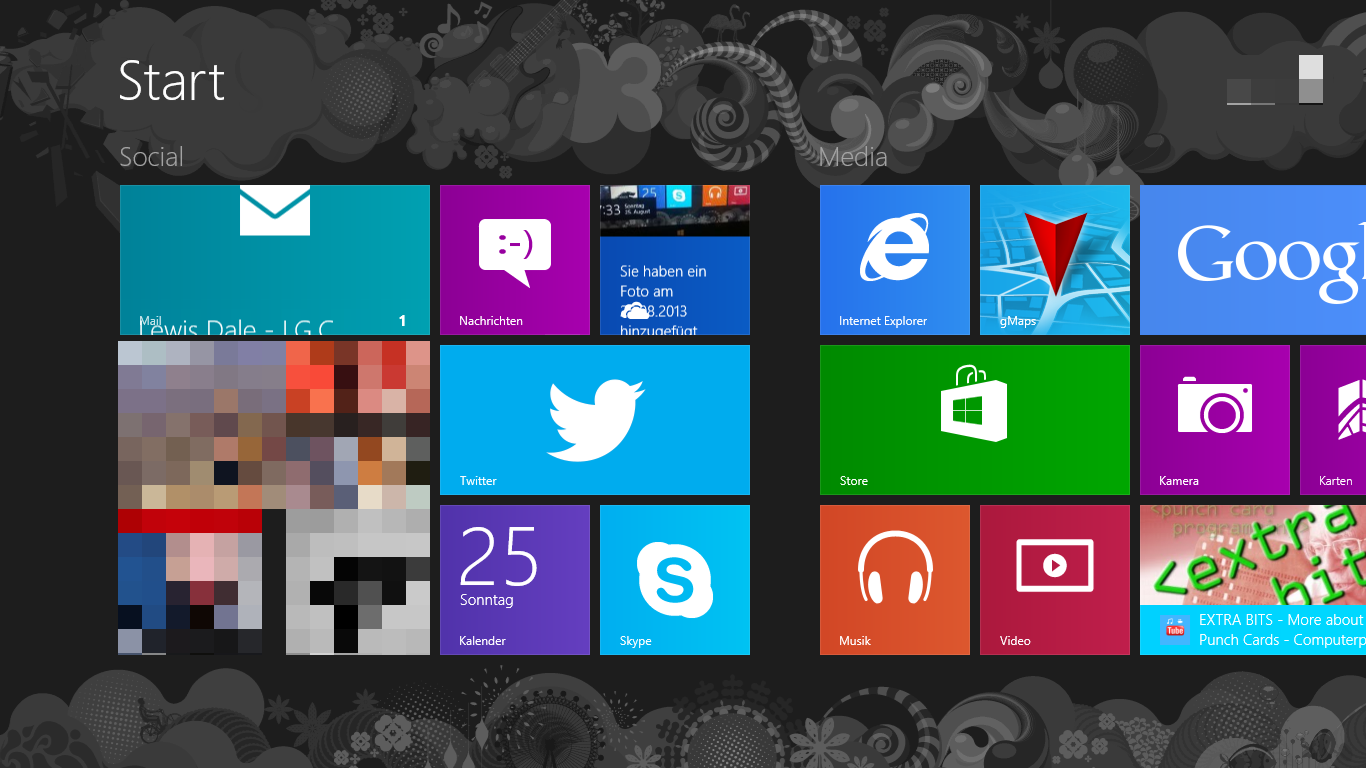
\includegraphics[width=0.6\textwidth]{Bilder/Screenshots/windows8/win8_startscreen.png} 
	\caption{Der Startbildschirm von Windows 8.}
	\label{fig:win8startscreen}
\end{figure}

Dies können Desktop-Programme oder Modern UI Apps (Windows-Store) sein, welche nur über den Microsoft Store zu installieren sind. Der bekannte Desktop-Modus ist in diesem Sinne auch \glqq nur\grqq\ ein spezielles Programm (App), welches in der neuen Oberfläche gestartet und ausgeführt werden kann.

Es gibt einige grundlegende Touch- und Mausgesten, um in der Modern UI Oberfläche zwischen den Apps zu navigieren oder um Optionen oder Einstellungen aufzurufen. Wenn sich der User auf einem Tablet befindet und über den rechten Bildschirmrand von rechts nach links wischt (swipen), öffnet sich am rechten Bildschirmrand die von Microsoft \glqq Charms\grqq\ genannte Menüleiste (siehe Abbildung \ref{fig:charms}). Hier befinden sich die Schaltflächen: Suchen, Teilen, Start , Geräte und Einstellungen. Um die Charms-Bar auf einem Gerät ohne Touch-Unterstützung aufzurufen, muss die Maus in die obere oder untere rechte Ecke des Bildschirms geführt werden. 

\begin{figure}[h]	
	\centering
	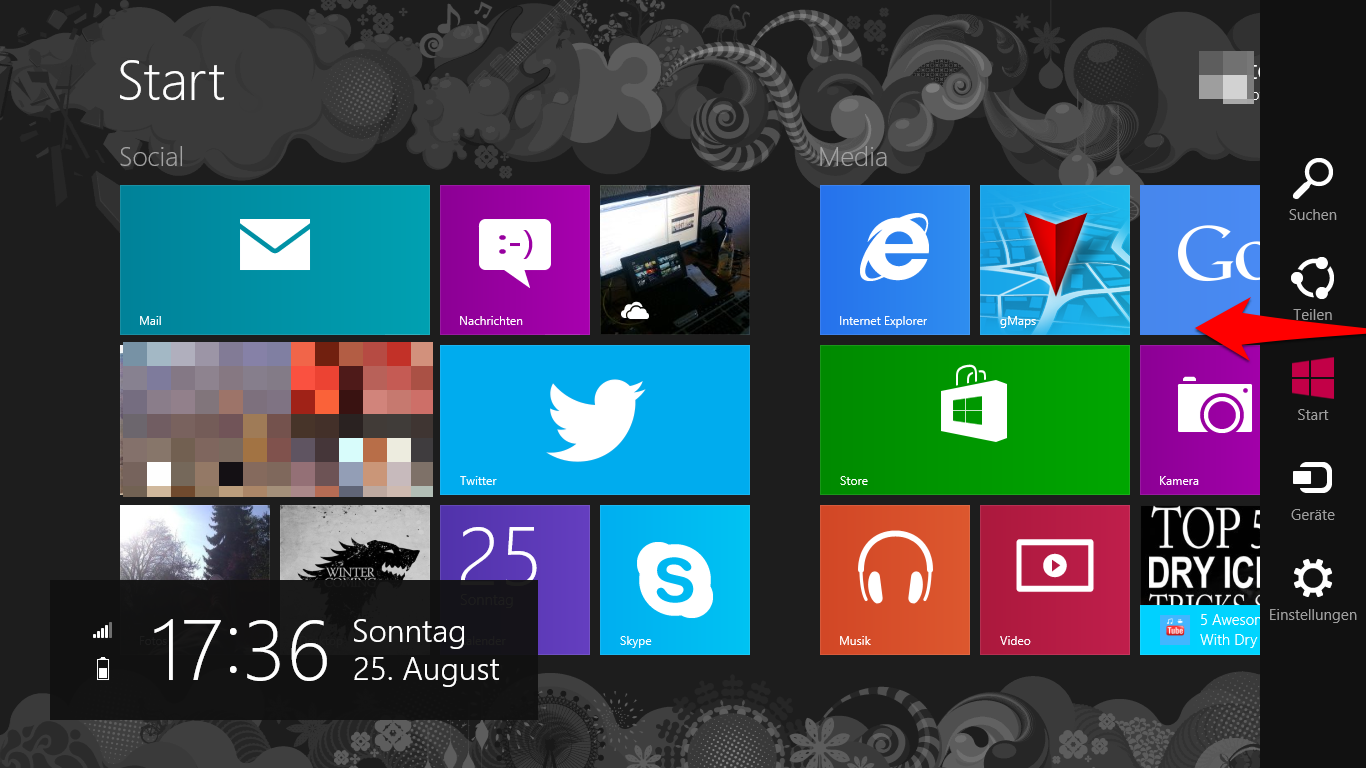
\includegraphics[width=0.6\textwidth]{Bilder/Screenshots/windows8/charm_bar.png} 
	\caption{Die Geste zum Aufrufen der Charms-Menüleiste.}
	\label{fig:charms}
\end{figure}  

Es können zwei verschiedene Gesten benutzt werden, um bequem zwischen den geöffneten Apps zu wechseln. Abbildung \ref{fig:appschanging} zeigt die beiden Möglichkeiten. Um eine Liste, wie sie die Abbildung auf der linken Seite darstellt, angezeigt zu bekommen, wird von links nach rechts über den linken Bildschirmrand gewischt. Anschließend wird ohne den Finger hochzunehmen zurück in Richtung des Bildschirmrandes gewischt. Bei der Bedienung mit der Maus wird die Maus zunächst in die obere oder untere linke Ecke bewegt, um anschließend nach unten bzw. nach oben zur Bildschirmmitte geführt zu werden.

Die zweite Möglichkeit besteht darin, die Apps direkt in der Reihenfolge, wie sie zuletzt aktiv waren, wieder in den Vordergrund zu bringen. Dazu wird von links nach rechts über den linken Bildschirmrand gewischt. Der rechte Teil von Abbildung \ref{fig:appschanging} zeigt diese Geste.
 
\begin{figure}[h]	
	\centering
	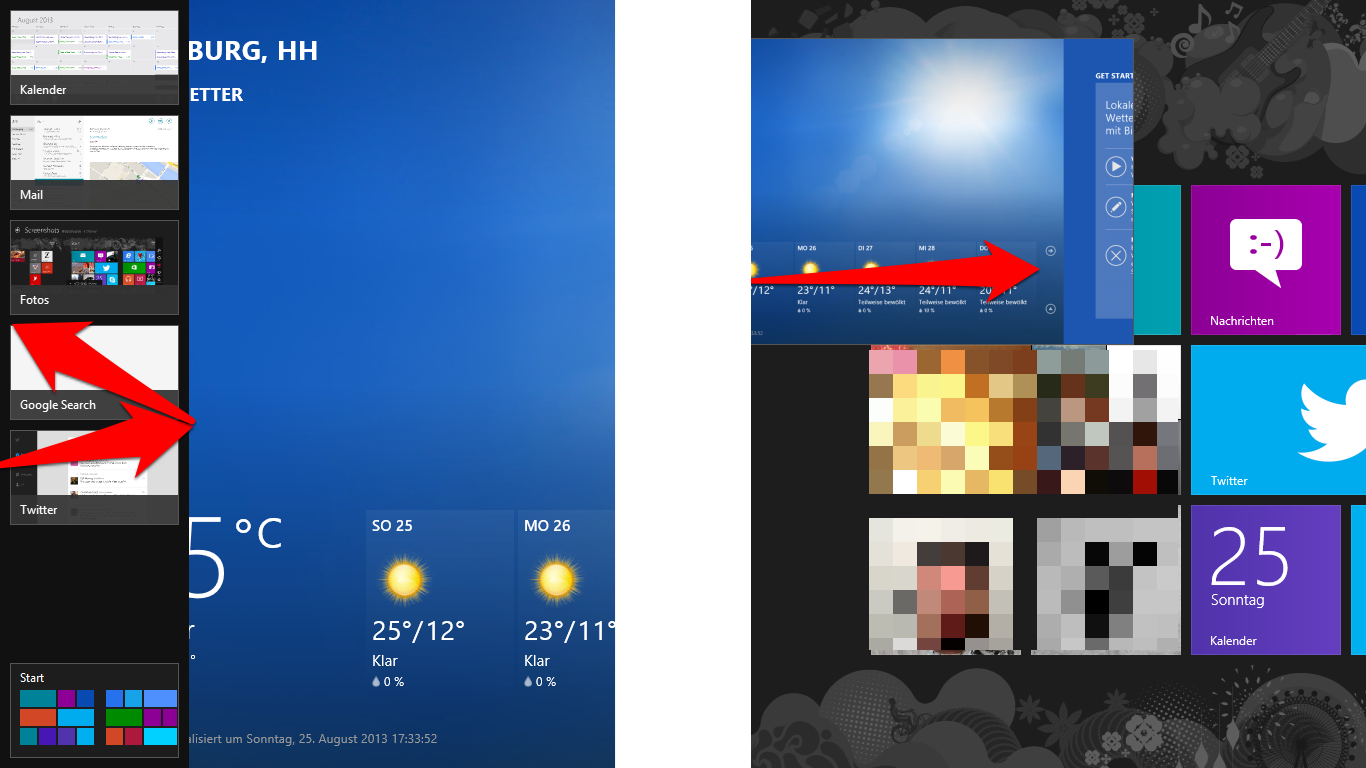
\includegraphics[width=0.6\textwidth]{Bilder/Screenshots/windows8/apps_changing.png} 
	\caption{Die Gesten zum Durchwechseln der Apps.}
	\label{fig:appschanging}
\end{figure}  

Die letzte grundlegende Geste wird benutzt, um z.B. Optionen, Einstellungen oder eine Navigationsleiste aufzurufen. Hierzu wird über den oberen oder den unteren Bildschirmrand in Richtung Bildschirmmitte gewischt. Wird diese Geste ausgeführt, öffnen sich die untere und die obere Menüleiste, unabhängig davon, ob der User die Geste am oberen oder am unteren Bildrand ausführt. Wenn es in der App oben und unten Menüleisten gibt, öffnen sich immer beide. Es ist nicht möglich, z.B. nur die obere Leiste zu öffnen. In der unteren Menüleiste befinden sich typischer Weise Einstellungen für die aktuelle Ansicht, in welcher sich die App gerade befindet. Sofern es eine Leiste am oberen Bildrand gibt, ist in dieser häufig eine Art von Navigation untergebracht. Abbildung \ref{fig:menubar} zeigt die obere und untere Menüleiste am Beispiel der vorinstallierten Wetter App.

\begin{figure}[h]	
	\centering
	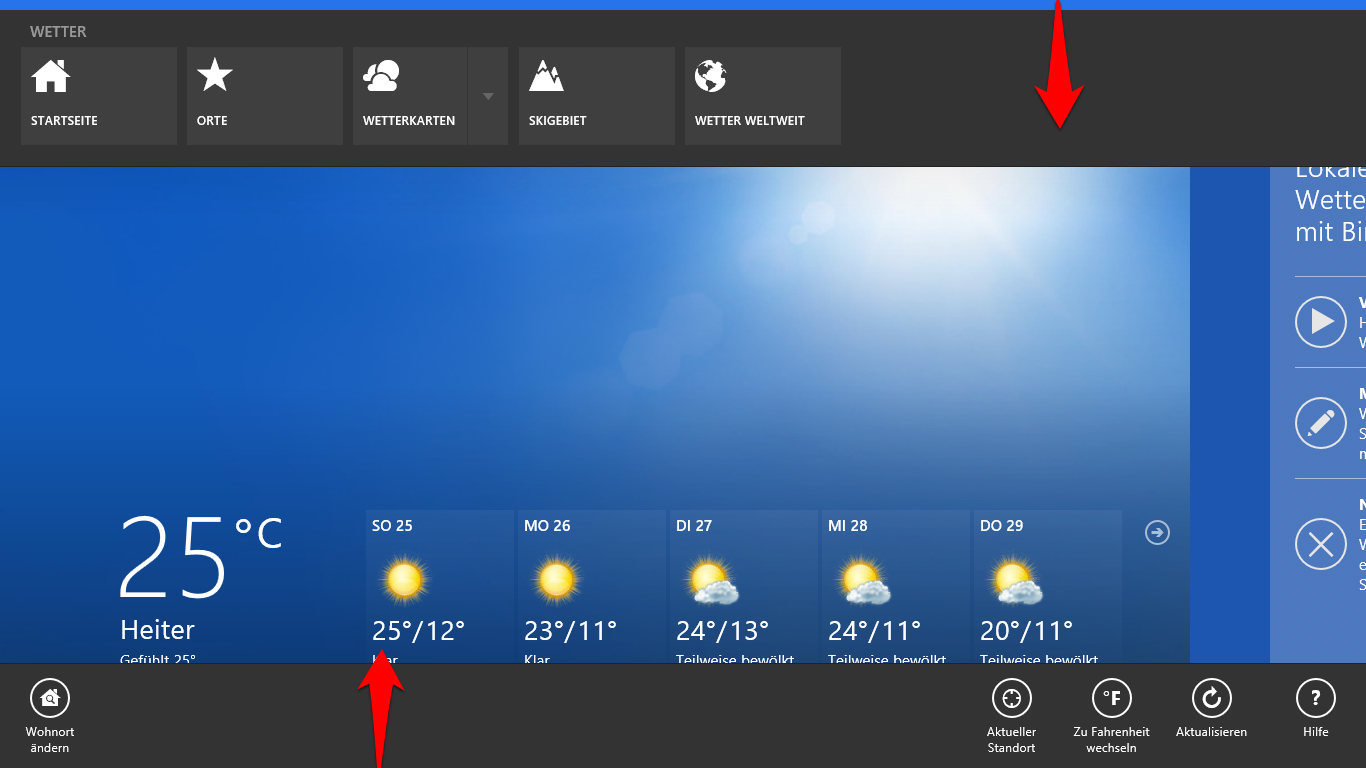
\includegraphics[width=0.6\textwidth]{Bilder/Screenshots/windows8/app_leisten.png} 
	\caption{Die Geste zum Öffnen der unteren und oberen Menüleiste.}
	\label{fig:menubar}
\end{figure}  

\subsection{Die Windows 8-Philosophie}
\label{subsec:win8philosophie}
% touch, vorteile, nachteile
Windows 8 ist wohl der radikalste Umbruch bei den Microsoft-Betriebssystemen seit Windows 95. Es sollen hier einige Aspekte beleuchtet werden, warum Microsoft diesen Weg eingeschlagen hat.

Viele Features, die heute mit einem Windows PC verbunden werden wie z.B. der Desktop, die Taskleiste oder das Startmenü, wurden ursprünglich in Windows 95 eingeführt. Damals hatte Windows noch keinen Browser. Mit der Zeit gewann das Internet immer mehr an Bedeutung, und der Browser rückte mehr und mehr in den Mittelpunkt der vernetzten Computernutzung. Das Betriebssystem hingegen veränderte sich kaum. Mit Windows 8 versucht Microsoft diesen Schritt nachzuholen und das Betriebssystem um den vernetzten User herum zu konzipieren. Eine der Hauptaufgaben übernehmen hierbei die sogenannten \textit{Live Tiles} auf dem Startbildschirm. Sie zeigen stets aktuelle Informationen, ohne dass der User den Browser öffnen muss \citep{Pachal2012}. 

\begin{quote}
\textit{There's tons of stuff on the Internet and your PC basically has this little straw — Internet Explorer — to see all this. We didn't think that should be the case. The whole PC should be about that. Part of what the Start screen is really about is making all this activity — these people that you care about, and all this information — sort of explode so you're immersed in it.} ---Sam Moreau\footnote{Director of design and research for Windows}
\end{quote}

Sam Moreau bringt es gut auf den Punkt. Es gibt so viel zu entdecken im Internet, doch bisher hatte der User nur einen kleinen \glqq Strohhalm\grqq\ , den Browser, um dies alles zu entdecken. Diese Funktion soll in Windows 8 der gesamte PC übernehmen. Alle Informationen, die dem User wichtig sind, sollten möglichst einfach einsehbar und erreichbar sein.

\subsection{Windows RT}
\label{subsec:winRT}
Windows RT ist ein separates Windows Betriebssystem, welches für PCs oder Tablets mit ARM-Architektur optimiert ist. Die größten Vorteile dieser Geräte sind normalerweise ein leichteres Gewicht und eine längere Akkulaufzeit gegenüber den Geräten, die mit einer x86/x64 Architektur ausgestattet sind. Auf den ersten Blick sieht Windows RT, von der Bedienoberfläche her, genau so aus wie Windows 8. Der größte und signifikanteste Unterschied zu Windows 8 ist jedoch der, dass aufgrund der ARM-Architektur auf Windows RT nur Programme und Apps aus dem Windows-Store installiert und ausgeführt werden können. Das Installieren von herkömmlichen Programmen, wie es Windows 8 zulässt, ist nicht möglich. Windows RT verfügt zwar über einen Desktop, wie er auch in Windows 8 vorhanden ist, allerdings laufen hier nur die vorinstallierten Office Produkte von Microsoft sowie der Microsoft Browser \textit{Internet Explorer}. Außerdem können nur speziell für Windows RT zertifizierte Geräte benutzt werden, das gilt u.a. auch für Mäuse und Tastaturen. \citep{MicrosoftWinRT}  
 
\subsection{Das Ökosystem}
\label{subsec:ökosystem}
Kaufte man früher einen PC, ein Notebook oder ein Handy, ging es bei der Abwägung der Kaufkriterien meist ausschließlich um Hersteller und Hardwarespezifikationen. In einer mehr und mehr mobilen und \textit{mehrgerätigen} Welt, wie wir sie heute erleben, kommt zu der Kaufentscheidung noch ein weiterer entscheidender Punkt hinzu. Welches Ökosystem passt am besten zu mir? Denn um auf mehreren Geräten wie z.B. Notebook, Tablet und Smartphone stets seine Daten aktuell und synchron zu halten, muss vorher genau bedacht werden, ob das gewählte Ökosystem den eigenen Anforderungen entspricht. Fragen, die zum  Ökosystem gestellt werden können, sind z.B.: Wie sieht es mit der Anzahl und Verfügbarkeit von Apps im jeweiligen Store aus? Gibt es eine Musikstreaming-Lösung? Wie sieht es mit Filmen und Büchern aus? Wie sehen die Dienste zum Speichern von Daten in der Cloud aus? Es fällt auf, dass heute nicht mehr nur ein Gerät gekauft wird, sondern dass zu diesem Gerät oder diesen Geräten meist ein ganzes Ökosystem mit geliefert wird, unabhängig davon, ob man sich für Apple, Google, Microsoft oder Amazon entscheidet. 

Mit der Einführung von Windows 8 hat Microsoft neuen Schwung in sein gesamtes Ökosystem gebracht. Es wurden verschiedene Dienste vereinheitlicht und zusammengefasst. Das Microsoft Ökosystem umfasst heute u.a. Windows 8, Windows RT, das Smartphone-Betriebssystem Windows Phone 8, den Cloudspeicherdienst Skydrive, den Streamingdienst xBox Music und den E-Mail Dienst outlook.com. Viele dieser Dienste existierten schon vor der Einführung von Windows 8. Aber erst mit dessen Einführung wurden die Dienste und Betriebssysteme einer einheitlichen \glqq Designkur\grqq\ unterzogen und enger aufeinander abgestimmt. Außerdem wird im Gegensatz zu vorher nur noch ein Benutzerkonto benötigt, um diese Dienste nutzen zu können.

\subsubsection{Windows Phone}
\label{subsubsec:windowsphone}
Windows Phone ist das Smartphone Betriebssystem von Microsoft. Die aktuelle Version ist Windows Phone 8. Es besitzt genau wie Windows 8 eine Kachel-Oberfläche. Obwohl Windows Phone 8 und Windows 8 auf dem gleichen Kernel basieren, können auf dem Smartphone keine Windows 8 Apps ausgeführt werden. Umgekehrt laufen Windows 8 Apps nicht unter Windows Phone. Auch beim Erstellen der Apps kann nicht gleichzeitig für beide Plattformen entwickelt werden. Abbildung \ref{fig:wp8} zeigt einen Startbildschirm von Windows Phone 8.

\begin{figure}[h]	
	\centering
	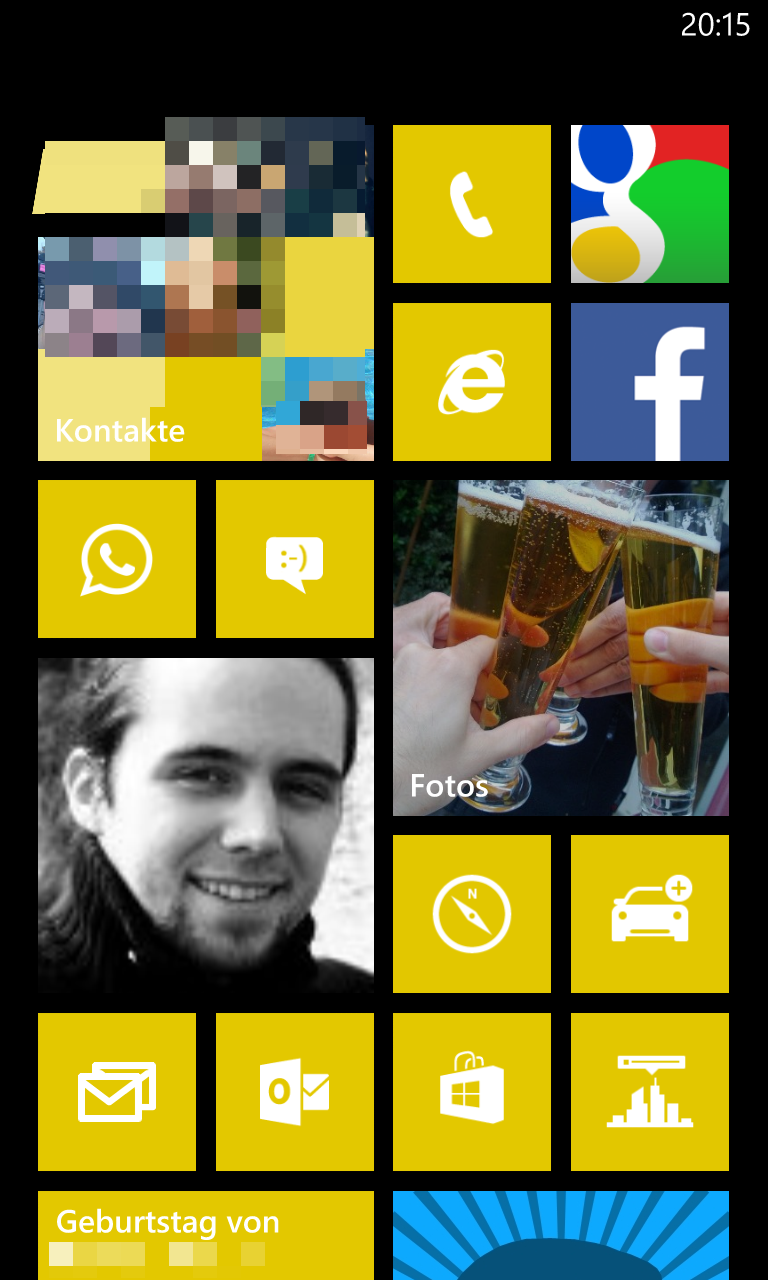
\includegraphics[width=0.25\textwidth]{Bilder/Screenshots/wp8/wp8_start.png} 
	\caption{Ein möglicher Startscreen von Windows Phone 8.}
	\label{fig:wp8}
\end{figure}  

\subsubsection{Microsoft App Stores}
\label{subsubsec:stores}
Eines der wichtigsten Elemente im Ökosystem eines Unternehmens ist der Store. Hier werden Apps für die Geräte mit dem jeweiligen Betriebssystem angeboten. Bei Apple ist es der \textit{App Store}, bei Google der \textit{Google Play Store} und bei Microsoft ist es  zum einen der \textit{Windows Store} für Windows 8- und Windows RT Apps und zum anderen der \textit{Windows Phone Store} für Smartphones mit Windows Phone. Oft fällt eine Entscheidung gegen ein bestimmtes Gerät aus der Windows-Welt mit der Begründung, es gäbe zu wenig Apps im Windows Store.

\begin{figure}[h]	
	\centering
	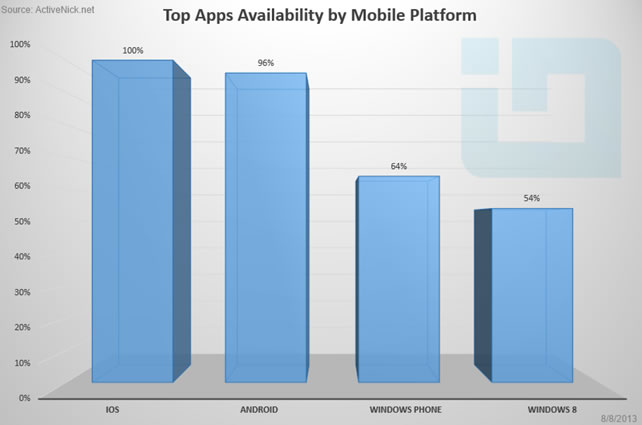
\includegraphics[width=0.8\textwidth]{Bilder/Abbildungen/store_chart.jpg} 
	\caption[Die Verfügbarkeit der Top 100 iOS Apps]{Verfügbarkeit der Top 100 iOS Apps auf anderen Systemen \citep{WinbetaStore2013}.}
	\label{fig:storechart}
\end{figure}  

Abbildung \ref{fig:storechart} zeigt die Verfügbarkeit der Top 100 iOS Apps \footnote{Liste: http://www.infragistics.com/community/blogs/nick-landry/archive/2013/08/06/top-100-apps-availability-on-ios-android-windows-phone-amp-windows-8.aspx} auf den anderen großen Systemen wie Android, Windows Phone und Windows 8. Hiernach sind im Windows Phone Store 64\% der Top 100 Apps vorhanden und im Windows 8 Store 54\%. Gezählt wurden hier nur offizielle Apps und keine Apps von Drittanbietern. In absoluten Zahlen hat iOS ca. 900.000 Apps im Appstore, Google über 1 Million Apps im Play Store, Windows Phone ca. 160.000 Apps und Windows 8 ca. 110.000 Apps im Windows Store \citep{WinbetaStore2013}.

Microsoft bemüht sich, die bekanntesten fehlenden Apps wie z.B. \textit{Instagram}, \textit{Pinterest}, \textit{Instapaper} oder \textit{Readability} schnellstmöglich nachzuliefern. Dabei wird den Entwicklern teilweise sogar Geld geboten, damit sie eine offizielle \glqq große\grqq\ App entwickeln \citep{WinbetaStore2013}.

\newpage
\section{Konzeption der App}
\label{sec:konzeption}
In diesem Abschnitt wird zunächst ein Blick auf die ZEIT ONLINE Webseite und auf bereits vorhandene ZEIT ONLINE Apps geworfen. Anschließend geht es darum, die Konzeption für eine Windows 8 Nachrichten App darzustellen und zu erläutern. Dabei gilt es darzulegen, warum und mit welchem Hintergrund Entscheidungen zu Gunsten der einen oder der anderen technischen oder konzeptionellen Methode ausfallen. Dazu müssen zunächst die Ziele der App dargelegt werden. Anschließend wird ein detaillierterer Blick auf das Herzstück der App geworfen, das Navigationskonzept. Hierbei ist eine der wichtigsten Fragen: \glqq Wie kann ich auch bei ggf. großen Datenmengen eine übersichtliche, intuitive Struktur schaffen, die sich in das Gesamtkonzept von Windows 8 eingliedert?\grqq. Zuletzt wird festgelegt, mit welcher Technologie bzw. Programmiersprache gearbeitet werden soll. 

Damit die zu erstellende App im Folgenden einen griffigeren Namen hat, wird an dieser Stelle die Namensfindung erläutert, sie heißt \glqq ZEIGHT\grqq\ (gesprochen: Zeit). Der Name setzt sich zusammen aus \glqq ZEIT\grqq\ und der englischen Zahl \glqq eight\grqq. Hintergrund ist, dass eine \glqq Zeit\grqq-App für Windows 8 (eight) entwickelt wird.

\subsection{ZEIT ONLINE}
\label{subsec:zeitonline}
ZEIT ONLINE ist das Internetangebot der Wochenzeitung DIE ZEIT. Berichtet wird über tagesaktuelle Ereignisse von einer eigenen Redaktion, die größtenteils in Berlin sitzt. Den Themenschwerpunkt bildet das Politik-Ressort. Um die ZEIT ONLINE Inhalte sowie auch die Inhalte der gedruckten ZEIT möglichst vielen Nutzern zugänglich zu machen, betreibt ZEIT ONLINE verschiedene Webseiten und Apps. Im folgenden soll ein  Überblick über die bereits vorhandenen Webseiten und Apps gegeben werden.

\subsubsection{Die Webseiten}
\label{subsubsec:webseiten}
Das Hauptaugenmerk bei ZEIT ONLINE liegt auf der herkömmlichen Webseite. Hier werden aktuelle Nachrichten dargestellt, die laufend aktualisiert werden.

\begin{figure}[h]	
	\centering
	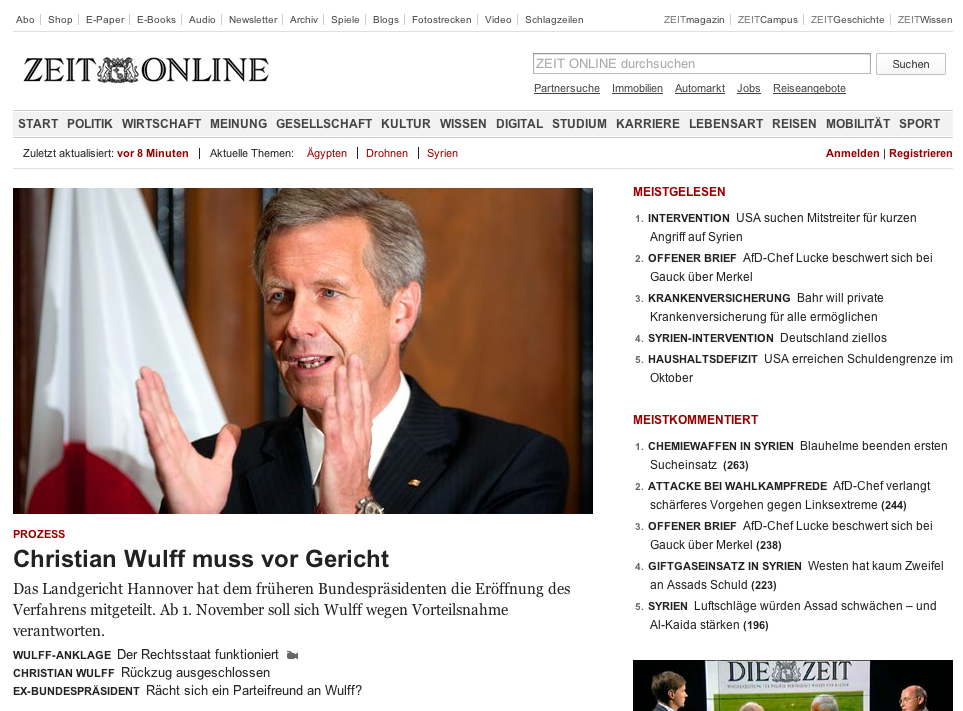
\includegraphics[width=0.6\textwidth]{Bilder/Screenshots/zeit.de/homepage.png} 
	\caption{Die Homepage von ZEIT ONLINE.}
	\label{fig:homepage}
\end{figure}

Abbildung \ref{fig:homepage} zeigt den obersten Teil der Homepage. Im oberen Bereich der Abbildung ist die Navigationsleiste zu erkennen. Sie zeigt die verschiedenen Haupt-Ressorts von ZEIT ONLINE. Klickt der User auf ein Ressort in der Navigation, landet er auf der jeweiligen sogenannten \textit{Centerpage} des Ressorts. Diese sieht im oberen Teil genauso aus wie die Homepage. Es gibt an erster Stelle ein großes Aufmacherbild oder Video und darunter meist mehrere kleinere \textit{Teaserelemente}. In der rechten Spalte sind die zurzeit meistgelesenen Artikel sowie die Artikel mit den meisten Nutzerkommentaren aufgelistet. Auf der Startseite gilt diese Liste über alle Ressorts hinweg, auf den jeweiligen Centerpages der Ressorts ist die Auflistung auf das jeweilige Ressort beschränkt.

Es gibt auf der ZEIT ONLINE Webseite nicht nur Nachrichtenbeiträge zu lesen. Daneben werden außerdem u.a. Bilderstecken, Videos, Spiele und Quizze angeboten. 

Da zunehmend immer mehr Leser die Webseite vom Smartphone aus aufrufen, gibt es unter \textit{mobil.zeit.de} eine für Smartphones optimierte mobile Webseite. In der Startansicht der mobilen Webseite werden alle Teaserelemente der Desktop Seite dargestellt. Außerdem werden darunter 3 Elemente aus jedem Ressort aufgeführt. Der Benutzer kann auch auf der mobilen Webseite direkt in ein Ressort wechseln und bekommt dort alle Elemente des jeweiligen Ressorts angezeigt. Auf Abbildung \ref{fig:mobilehomepage} sind von links nach rechts, die Startseite, die Artikelansicht und das Navigationsmenü für die Ressorts dargestellt.

\begin{figure}[h]	
	\centering
	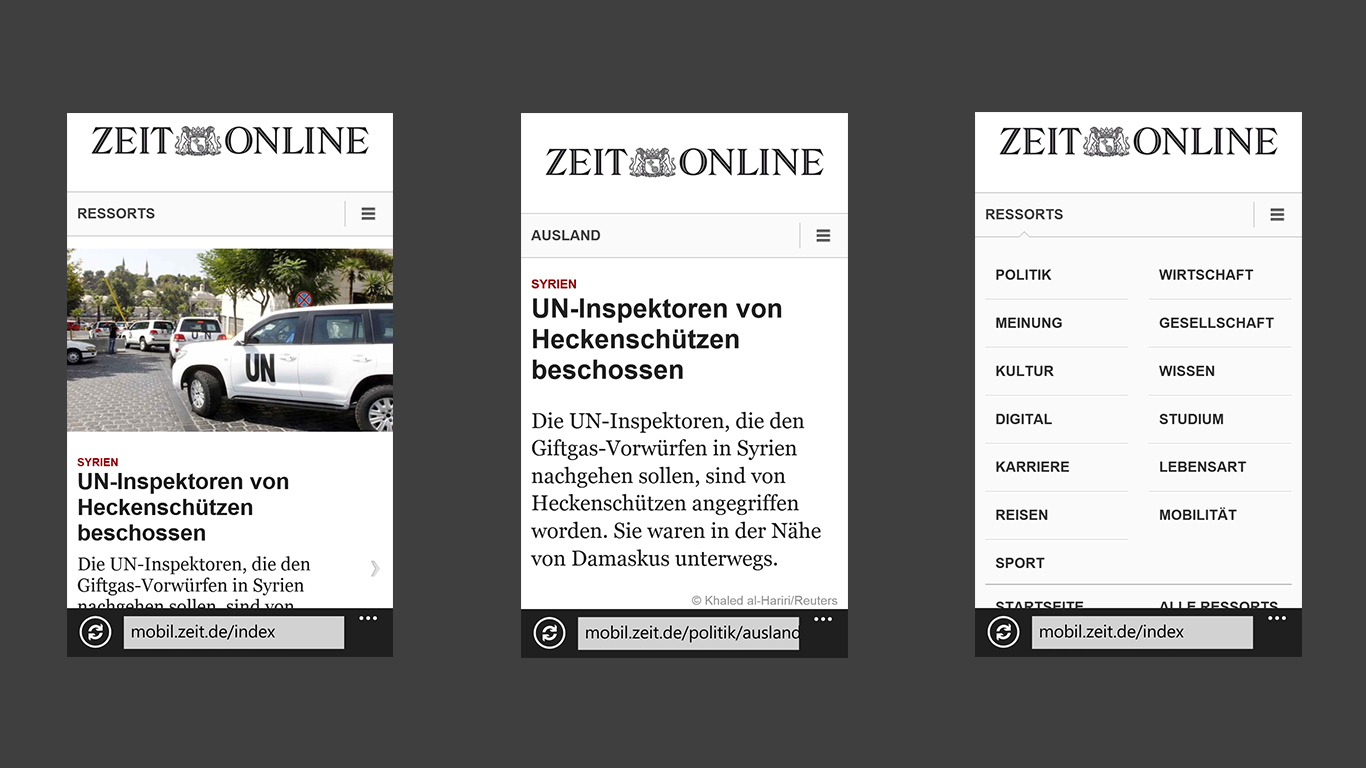
\includegraphics[width=\textwidth]{Bilder/Screenshots/mobil.zeit.de/mobile.png} 
	\caption{Die mobile Webseite von ZEIT ONLINE.}
	\label{fig:mobilehomepage}
\end{figure}

\subsubsection{Die iPad App}
\label{subsubsec:ipadapp}
Neben den ZEIT ONLINE Webseiten existieren mehrere Apps für verschiedene Geräte. Dazu gehört auch die App für das iPad von Apple. In der iPad App können keine Inhalte von ZEIT ONLINE angesehen werden. Stattdessen bietet sie jede Woche die digitale Ausgabe der gedruckten ZEIT und das ZEIT Magazin an. Die Ausgaben können sowohl im Abonnement als auch einzeln erworben werben. Eine eigene iPad Redaktion bereitet jede Woche die Artikel der gedruckten Ausgabe der ZEIT für die digitale Ansicht auf. Es werden z.B. Fotostrecken oder Audiokommentare mit eingebunden.  

\begin{figure}[h]	
	\centering
	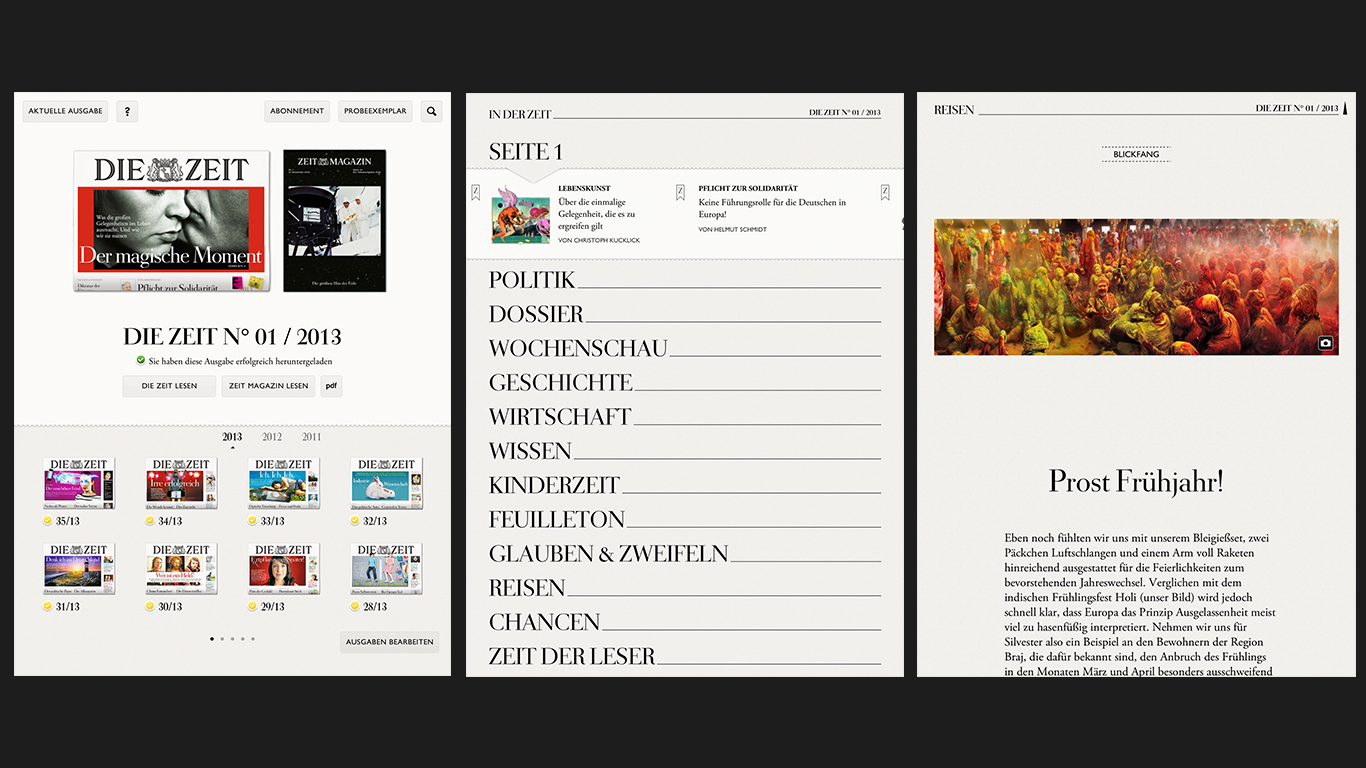
\includegraphics[width=\textwidth]{Bilder/Screenshots/iPadApp/ipad1.png} 
	\caption[Die iPad App]{Die iPad App zeigt die aufbereiteten Artikel der gedruckten Ausgabe der ZEIT.}
	\label{fig:ipad1}
\end{figure}

Abbildung \ref{fig:ipad1} zeigt links die Ausgabenverwaltung der App. Hier können die Ausgaben erworben und heruntergeladen werden. In der Mitte ist das Inhaltsverzeichnis dargestellt. Hier ist gut zu sehen, in wieweit sich die Ressorts von ZEIT ONLINE und DIE ZEIT unterscheiden. Rechts auf der Abbildung ist ein zufälliger Artikel zu sehen. Findet der User einen Artikel interessant oder möchte ihn zum späteren Lesen speichern, kann er ihn im Bereich \textit{Meine Zeit} ablegen. 

\subsubsection{Die Webapp}
\label{subsubsec:webapp}
Eine weitere App ist die Webapp. Sie ist im Grunde eine abgespeckte Version der iPad App. Es können ebenfalls keine ZEIT ONLINE Inhalte konsumiert werden, sondern nur die digitalen Ausgaben der ZEIT erworben werden. Die Webapp ist im Browser unter \textit{webapp.zeit.de} erreichbar. Des Weiteren gibt es einen Android- und einen Kindle-Wrapper, sodass die App auch über den \textit{Google Play Store} sowie den \textit{Amazon Store} zu beziehen ist. 

\begin{figure}[h]	
	\centering
	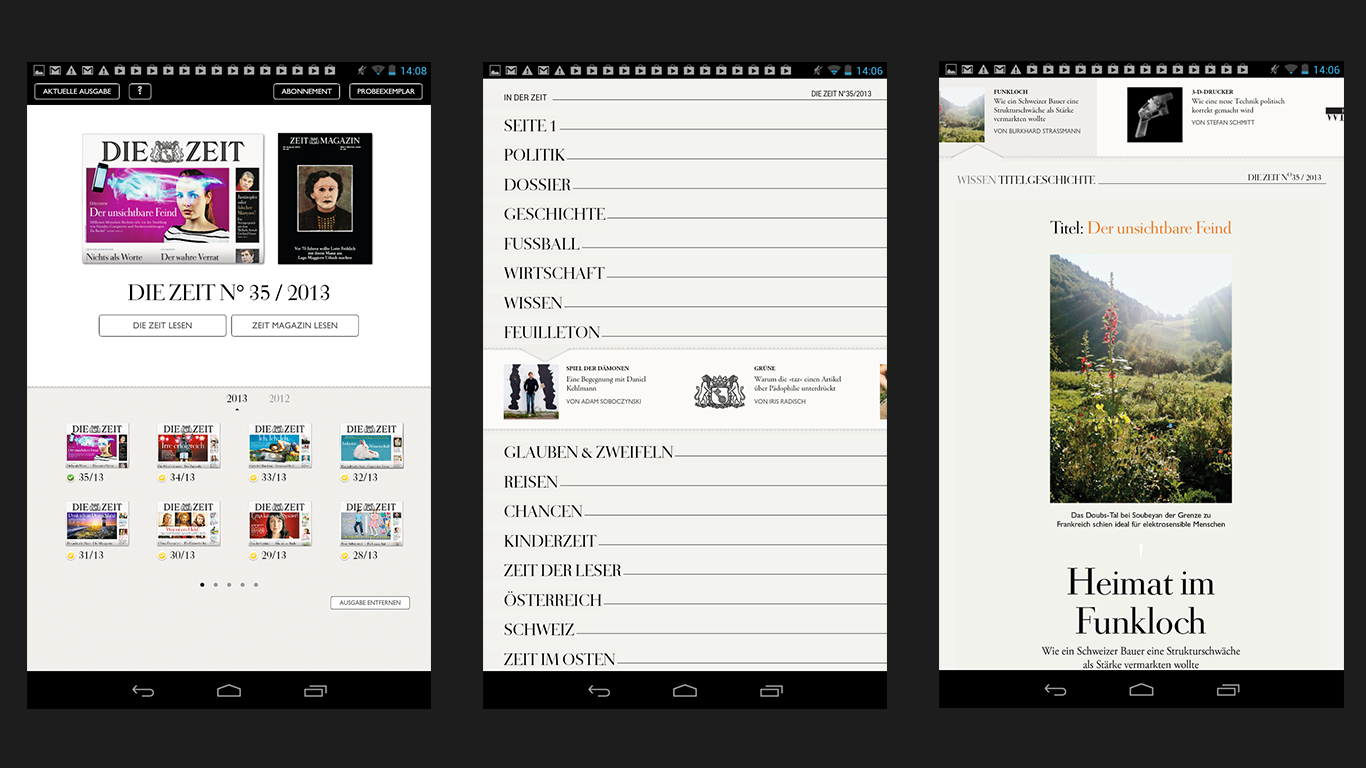
\includegraphics[width=\textwidth]{Bilder/Screenshots/android-webapp/webapp.png} 
	\caption[Die Webapp]{Die Webapp zeigt genau wie die iPad App die aufbereiteten Artikel der gedruckten ZEIT.}
	\label{fig:webapp}
\end{figure}

Abbildung \ref{fig:webapp} zeigt die Webapp auf einem Android Tablet (Nexus 7). Auf den ersten Blick scheint sie identisch mit der iPad App. In der Webapp können jedoch keine Lesezeichen, wie es in der iPad App möglich ist, gesetzt werden. Außerdem kann hier aus einem Artikel heraus nicht direkt in ein Ressort gesprungen werden. Auch dies ist bei der iPad App möglich.

\subsubsection{Die iPhone App}
\label{subsubsec:iphoneapp}
In der iPhone App werden dem User sowohl Inhalte von ZEIT ONLINE als auch die digitale PDF-Ausgabe der gedruckten Zeit angeboten.

\begin{figure}[h]	
	\centering
	\includegraphics[width=\textwidth]{Bilder/Screenshots/iPhoneApp/iPhone.png} 
	\caption[Die iPhone App]{Die iPhone App zeigt sowohl Inhalte von ZEIT ONLINE als auch von der ZEIT.}
	\label{fig:iphoneapp}
\end{figure}

Die inhaltliche Struktur ähnelt der der mobilen Webseite. Allerdings kann der User die iPhone App nach seinen Vorlieben anpassen. So kann z.B. eingestellt werden, wie viele Artikel pro Ressort auf der Startseite angezeigt werden sollen.

Abbildung \ref{fig:iphoneapp} zeigt eine Bilderstrecke der iPhone App. Das zweite Bild von links zeigt einige der möglichen Einstellungen, die der User vornehmen kann. Das Bild ganz rechts zeigt ein weiteres Feature der App. Es können ausgewählte Artikel heruntergeladen werden und so für den Offline-Betrieb gespeichert werden.

\subsection{Ziele der App - Was wird dargestellt}
\label{subsec:zielderapp}
Das übergeordnete Ziel der ZEIGHT App ist es, eine Nachrichten Applikation für Windows 8 zu erstellen, die den Inhalt der ZEIT ONLINE Webseite auf für den Nutzer ansprechende und intuitive Art und Weise darstellt. Das Layout und die Darstellung der Inhalte sollen sich an das sogenannte \glqq Look and Feel\grqq\ von Windows 8 anpassen und sich daran orientieren.

Der Fokus bei den Inhalten liegt auf den Artikeln selbst und den jeweiligen Aufmacher bzw. Teaser Bildern. Andere Inhalte wie z.B. Bildergalerien, Infografiken, Blogartikel oder Quizze werden von der App nicht erfasst und nicht dargestellt, da es in der Fragestellung schwerpunktmäßig um die Relation zwischen den Aufmacherbildern und den dahinter liegenden Artikeltexten geht. Die App erhebt in dieser Hinsicht keinen Anspruch darauf, die gesamten redaktionellen Inhalte von \mbox{ZEIT ONLINE} darzustellen, sondern versteht sich eher als explorative Applikation im Sinne der Fragestellung.

Gleichzeitig soll eine Umgebung geschaffen werden, die es erlaubt Untersuchungen anzustellen, inwieweit es möglich ist, allein durch das Betrachten der Aufmacherbilder auf den Inhalt der jeweiligen Artikel zu schließen (siehe Abschnitt \ref{subsubsec:nurbildermodus} auf Seite \pageref{subsubsec:nurbildermodus}). Der User soll die Möglichkeit haben, die standardmäßig vorhandenen Artikeltitel auszublenden, um so, wenn gewünscht, einen rein visuellen Eindruck der Artikelbilder zu bekommen.

Außerdem soll ZEIGHT dazu dienen zu erforschen, wie eine Nachrichten App in der Modern UI Oberfläche von Windows 8 erstellt wird und welche design- und auch funktionstechnischen Vorgaben von Microsoft vorhanden sind, das heißt wie eine App mit Nachrichteninhalten aus Microsofts Sichtweise auszusehen hat.

Zusammengefasst soll eine Windows 8 App erstellt werden, welche die Artikel der ZEIT ONLINE Webseite darstellt. Dieses übergeordnete Ziel umfasst drei Teilziele.

\begin{enumerate}
	\item Das User Interface der App ist ansprechend gestaltet
	\begin{itemize}
		\item Look \& Feel entspricht Windows 8
		\item Die Nutzer können die App intuitiv bedienen
	\end{itemize}
	\item Die Umsetzung eines \glqq Nur-Bilder-Modus\grqq\ ist vorhanden
	\item Für zukünftige Windows 8 Entwicklungen bei ZEIT ONLINE ist Know How über die App-Entwicklung mit Webtechnologien vorhanden
\end{enumerate}


\subsection{Graphical User Interface}
\label{subsec:gui}
Damit der User ein für ihn angenehmes und flüssiges Nutzungserlebnis hat, ist es notwendig, sich über das \ac{gui} Gedanken zu machen, gerade wenn es sich um eine App handelt, in der es viele verschiedene Inhaltsbereiche gibt. Der User soll sich möglichst intuitiv durch die Inhalte bewegen können. Außerdem muss dem User auf der Einstiegsebene ein guter Überblick über die vorhandenen Inhalte gegeben werden, damit er von dort aus zielgerichtet weiter navigieren kann, ohne lange suchen zu müssen. Hierzu ist muss ein passendes Navigationskonzept gefunden werden.  Microsoft nennt in seinen Richtlinien für Windows Store Apps (Modern UI Apps) grundsätzlich zwei Möglichkeiten, wie die Navigation umgesetzt werden kann. Diese werden nachfolgend beschrieben.

\subsubsection{Flaches Navigationssystem}
\label{subsubsec:flachessystem}
Das flache Navigationssystem wird in vielen Windows Store Apps verwendet, häufig in Spielen, Browsern oder in Apps zum Erstellen von Dokumenten. Es zeichnet sich dadurch aus, dass sich die Inhalte auf der gleichen hierachischen Ebene befinden. Dieses System eignet sich dann, wenn ein schneller Wechsel zwischen wenigen Seiten oder Registerkarten möglich sein soll \citep{MicrosoftNavidesign2013}.

\begin{figure}[h]	
	\centering
	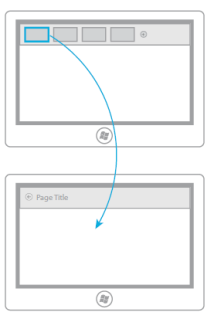
\includegraphics[scale=1]{Bilder/Abbildungen/ms_navigation_flach.png} 
	\caption[Das flache Navigationssystem]{Das flaches Navigationssystem \protect\citep{MicrosoftNavidesign2013}.}
	\label{fig:naviflach}
\end{figure}

Abbildung \ref{fig:naviflach} zeigt, wie das flache Navigationssystem funktioniert. Am oberen Rand befindet sich eine nicht immer sichtbare Navigationsleiste mit den verschiedenen Registerkarten oder Seiten. Die Leiste wird angezeigt, wenn der User vom unteren oder oberen Bildrand wischt (siehe Abschnitt \ref{subsec:bedienkonzept}). Wenn der User die Seite wechseln möchte, geschieht dies  direkt über die Navigationsleiste, d.h. es gibt meist keinen permanenten Zurück-Button. 

Ein flaches Navigationssystem eignet sich nicht für eine Nachrichten App wie die, die in dieser Arbeit konzipiert und umgesetzt werden soll, weil es zu viele Bereiche (Ressorts) gibt, die sich strukturell zudem sehr ähneln. Hier ist es angebracht, ein hierarchisches Navigationssystem zu verwenden.    


\subsubsection{Hierarchisches Navigationssystem}
\label{subsubsec:hierachischessystem}
Die meisten Windows Store-Apps benutzen ein hierarchisches Navigationssystem, Microsoft nennt es Hubnavigationsmuster. Es ist geeignet, um große Inhaltssammlungen zu ordnen und sie für User benutzerfreundlich aufzubereiten. Der Schlüssel dazu ist die Unterteilung des Inhalts in verschiedene Detailebenen \citep{MicrosoftNavidesign2013}.

\begin{figure}[h]	
	\centering
	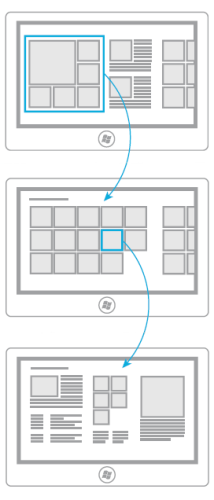
\includegraphics[scale=1]{Bilder/Abbildungen/ms_navigation_hierarchie} 
	\caption[Das flache Navigationssystem]{Das hierarchisches Navigationssystem \protect\citep{MicrosoftNavidesign2013}.}
	\label{fig:navihierarchisch}
\end{figure}

Das Schema eines hierarchischen Systems ist in Abbildung \ref{fig:navihierarchisch} dargestellt. Der Einstiegspunkt in die App ist die sogenannte \glqq Hubansicht\grqq, hier ganz oben in der Abbildung zu sehen. In der Hubansicht wird aus den vielen großen Bereichen der App jeweils ein kleiner Teil gesammelt und dargestellt, sodass sich der User vorstellen kann, was ihn im jeweiligen Bereich erwartet. Die Anordnung, in welcher der Auszug der Inhalte dargestellt ist, muss nicht für alle Bereiche gleich sein, es können verschiedene Templates für den Seitenaufbau hinterlegt werden. Es kann das Nutzungserlebnis verbessern und vielfältiger gestalten, wenn unterschiedliche Darstellungen z.B. in Höhe, Breite oder Anzahl der Objekte für die Bereiche genutzt werden. Die Hubansicht wird horizontal gescrollt, d.h. weiterer Inhalt befindet sich hinter dem rechten Rand und kann entweder durch das Scrollrad der Maus oder auf einem Tablet durch das Swipen nach links in das Sichtfeld des Users gebracht werden.

Die mittlere Darstellung in Abbildung \ref{fig:navihierarchisch} zeigt die zweite Detailstufe des hierarchischen Systems. Hier werden alle Elemente eines Bereichs dargestellt.

Im unteren Bereich der Abbildung ist schließlich die letzte Detailstufe zu sehen. Es handelt sich hierbei um den eigentlichen Inhalt, z.B. einen Artikel. Es ist ebenfalls möglich, von der Hubansicht direkt in die Detailansicht eines Elements zu wechseln.  

\begin{figure}[h]	
	\centering
	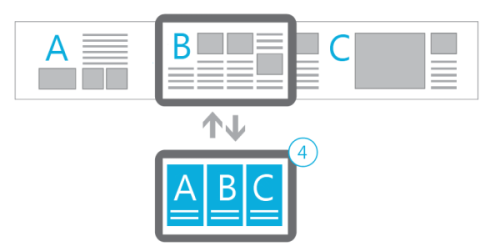
\includegraphics[scale=1]{Bilder/Abbildungen/ms_navigation_hierarchie_semantic_zoom} 
	\caption[Das Schema des \glqq Semantic Zoom\grqq]{Das Schema des \glqq Semantic Zoom\grqq\ \protect\citep{MicrosoftNavidesign2013}.}
	\label{fig:semanticzoomkonzept}
\end{figure}

Befinden sich in der Hubansicht, trotz der Zusammenfassung der Bereiche noch zu viele Bereiche und es dauert zu lange, bis zum Ende der Darstellung zu scrollen, kann noch eine weitere Ebene \glqq davor\grqq\ gelegt werden. Das Konzept nennt Microsoft \glqq Semantic Zoom\grqq\ und ist in Abbildung \ref{fig:semanticzoomkonzept} schematisch dargestellt. Oben in der Abbildung ist die Hubansicht dargestellt, unten die zusätzliche \glqq Semantic Zoom\grqq\ Ebene. In der Praxis kann der User auf diese Weise die Inhalte noch weiter vereinfachen und zusammenfassen lassen. Im Fall dieser App soll es einen semantischen Zoom geben, um ein flüssigeres und schnelleres Navigieren z.B. ganz zum Ende der Hubansicht zu ermöglichen, da es wahrscheinlich über zehn verschiedene Ressorts geben wird. Um am Desktop-PC mit Maus diese Ansicht aufzurufen, muss der User auf ein kleines Minuszeichen am unteren rechten Rand klicken. Am Tablet wird der semantische Zoom mit der \glqq Pinch to Zoom (out)\footnote{Zwei Finger (Berührungspunkte), die sich auf dem Bildschirm auf einander zu bewegen.}\grqq\  Geste aufgerufen. Klickt der User auf ein Element in dieser zusätzlichen Navigationsebene, wird er direkt zum jeweiligen Ausschnitt in die Hubansicht navigiert. Die \glqq Semantic Zoom\grqq\ Ansicht kann von jedem Punkt aus der Hubansicht aufgerufen werden.  

\subsubsection{Menü und Features}
\label{subsubsec:menuandproperties}
Da die ZEIGHT App einen explorativen Charakter hat, werden die Funktionen und Features auf das Nötigste beschränkt. Es soll eine untere App-Leiste geben, in der in Abhängigkeit von der gerade gewählten Ansicht verschiedene Optionen angezeigt werden. Diese Leiste ist nicht dauerhaft zu sehen und kann durch einen Rechtsklick aufgerufen werden, falls mit der Maus gearbeitet wird. Auf einem Tablet geschieht dies durch Swipen vom oberen oder unteren Bildschirmrand.

In der Startansicht sowie in der Ressortübersicht soll es am unteren Bildrand die Möglichkeit geben, die Titel aller Elemente aus- bzw. auch wieder einzublenden, um so dem User alternativ ein rein visuelles Erleben der Artikelbilder zu ermöglichen. In der Artikelansicht soll der User die Möglichkeit haben, die Schriftgröße des Artikels zu vergrößern, zu verkleinern oder wieder auf ihren Startwert zu setzen, da die App eventuell auf Monitoren mit verschieden großen Auflösungen ausgeführt wird oder die Sehkraft des Users nicht mehr ausreicht, um eine normal große Schrift zu erkennen und zu lesen. So wird ein gewisses Maß an Barrierefreiheit gewährleistet. 


\subsection{Umsetzungsmöglichkeiten in Visual Studio}
\label{subsec:nativ_vs_web}
Vor dem Entwickeln einer Windows 8 App muss entschieden werden, mit welcher Technologie bzw. mit welcher Programmiersprache entwickelt werden soll. Die Rede ist hier von einer App, die in der Modern UI Oberfläche von Windows 8 läuft und für diese konzipiert ist. Es handelt sich nicht um eine klassische .NET oder WIN32 Anwendung für Windows. Um eine Modern UI App zu entwickeln, müssen zwei Dinge zwingend vorhanden sein. Zum einen wird Windows 8 selbst und zum anderen die neueste Version von Visual Studio, Visual Studio 11\footnote{Visual Studio 2011 war die aktuellste Version beim Erstellen dieser Arbeit.}, benötigt. Visual Studio steht in der Express Version für Windows 8 kostenlos zur Verfügung. Des Weiteren muss zwischen der nativen Umsetzung und der Implementierung mit Webtechnologien entschieden werden. Es soll zunächst erläutert werden, was die beiden Begriffe bedeuten und in welcher Weise und welchem Zusammenhang sie bei der Entwicklung einer Windows 8 Modern UI App üblicherweise gebraucht werden.

\subsubsection{Native App}
\label{subsubsec:nativ}
Der heutige Begriff \glqq native App\grqq\ unterscheidet sich in einigen Punkten von der früheren oder ursprünglichen Verwendung des Begriffs. Früher sprach man von einer nativen App, wenn direkt auf die Ressourcen der  Maschine zugegriffen wurde, wie z.B. Maschinencode, der direkt von der CPU ausgeführt wird. Heute wird eine App oftmals schon als nativ deklariert, wenn es sich nicht um eine Webapp handelt. Eine sinnvolle Definition liegt zwischen diesen beiden Varianten. Eine App ist dann nativ, wenn sie geräte- , betriebssystem- oder laufzeitumgebungsabhängig ist. Sie ist für ein spezielles Gerät entwickelt und kann nur auf diesem ausgeführt werden. Dabei kann sie alle geräte- oder betriebssystemspezifischen Funktionen nutzen, es ist jedoch nicht relevant wie nah an der Hardware tatsächlich programmiert wurde \citep{OBrian2013}.

In Visual Studio können native Windows 8  Apps u.a. mit den Programmiersprachen C++, C\# oder Visual Basic erstellt werden. Für das Design bzw. das Aussehen der App wird die Markupsprache - \ac{xaml} - verwendet. Es gibt zwei Möglichkeiten, wie das \ac{xaml} erstellt werden kann. Es kann entweder von Hand geschrieben oder automatisch generiert werden. Zum automatischen Generieren lassen sich per Drag \& Drop Elemente wie z.B. Buttons und andere Schaltflächen aus einer Werkzeugpalette direkt auf die \glqq App-Leinwand\grqq\ ziehen und dort verschieben oder nach Belieben anordnen.

\subsubsection{Windows 8 App mit Webtechnologien}
\label{subsubsec:webwin8}
In Visual Studio können nicht nur Apps mit den klassischen Programmiersprachen, wie im vorigen Abschnitt beschrieben, erstellt werden. Visual Studio erlaubt es, Apps mit Webtechnologien zu erstellen. So können Apps mit \ac{html}, CSS und JavaScript erstellt werden. Das Markup wird mit \ac{html} erstellt, dieses dann mit CSS gestylt und die Programmlogik mit JavaScript realisiert. Die resultierende App ist trotzdem eine native Windows 8 Anwendung und kann nur auf Windows 8 oder Windows RT Geräten installiert und ausgeführt werden. Das Design und das Layout einer solchen App können in Visual Studio allerdings nicht visuell oder per Drag \& Drop entworfen werden. Für diesen Zweck liefert Microsoft ein gesondertes Programm mit, \textit{Blend für Visual Studio 2012}. In Blend können \ac{html} und CSS Änderungen direkt in einer Live-Vorschau angesehen werden. Außerdem können hier auch Elemente per Drag \& Drop angeordnet und verschoben werden. Ein geöffnetes Visual Studio Projekt kann mit zwei Klicks im Menü direkt in Blend geöffnet werden. 

Auf diese Weise wird es Webentwicklern ermöglicht, einen komfortablen Einstieg in die Programmierung von Windows 8 Apps zu finden. Damit bleibt die Entwicklung nicht nur den .NET-Entwicklern vorbehalten. Ganz ohne Lernaufwand kommen allerdings auch die Webentwickler nicht aus. Um eine App mit Webtechnologien erstellen zu können, müssen sich die Entwickler zuvor mit der neuen API-Technologie vertraut machen \citep{Bleske2012}.

Das Hauptaugenmerk liegt hierbei auf Microsofts hauseigener JavaScript-Bibliothek \textit{\ac{winjs}}. Sie bietet viele wichtige Funktionen z.B. zur Handhabung von Steuerelementen oder zu Behandlung von großen Datenmengen. 

Letztendlich macht es keinen großen Unterschied, ob mit herkömmlich Programmiersprachen oder mit Webtechnologien gearbeitet wird. Viele Apps lassen sich mit beiden Ansätzen gleich gut umsetzen. Da die Entwicklung von nativen Apps mit Webtechnologien ein neues und interessantes Konzept ist, soll es in dieser Arbeit ausprobiert und angewandt werden.

\newpage
\section{Umsetzung der App}
\label{sec:umsetzungderapp}
Nachdem die Konzeption der ZEIGHT App abgeschlossen ist, wird in diesem Abschnitt erläutert, wie die App umgesetzt wird. Dazu wird zunächst Microsofts Raster-Vorlage näher beleuchtet. Anschließend werden die Datenanbindung, die Darstellung der Daten sowie die Features erklärt. Am Ende dieses Abschnitts befindet sich die Entwicklungschronologie. Sie gibt einen detaillierten Einblick in den zeitlichen Ablauf der einzelnen Entwicklungsschritte.

\subsection[Rastervorlage] {Rastervorlage\footnote{Die Namen der verwendeten Dateien in der Rastervorlage wurden mittlerweile von Microsoft geändert.}}
\label{subsec:rastervorlage}
Beim Erstellen einer Windows 8 Modern UI App mit \ac{html} und JavaScript bietet Microsoft von Haus aus verschiedene Vorlagen für Visual Studio, welche schon einige Grundfunktionen besitzen und sich so als guter Startpunkt für eine weiterführende App eignen. Die Vorlage, die für diese App verwendet wird, ist die Raster-App (engl. Grid Application) Vorlage. Sie bietet die Grundarchitektur für ein hierarchisches Navigationssystem wie es in Abschnitt \ref{subsubsec:hierachischessystem} auf Seite \pageref{subsubsec:hierachischessystem} beschrieben ist.

\begin{figure}[h]
	\centering
	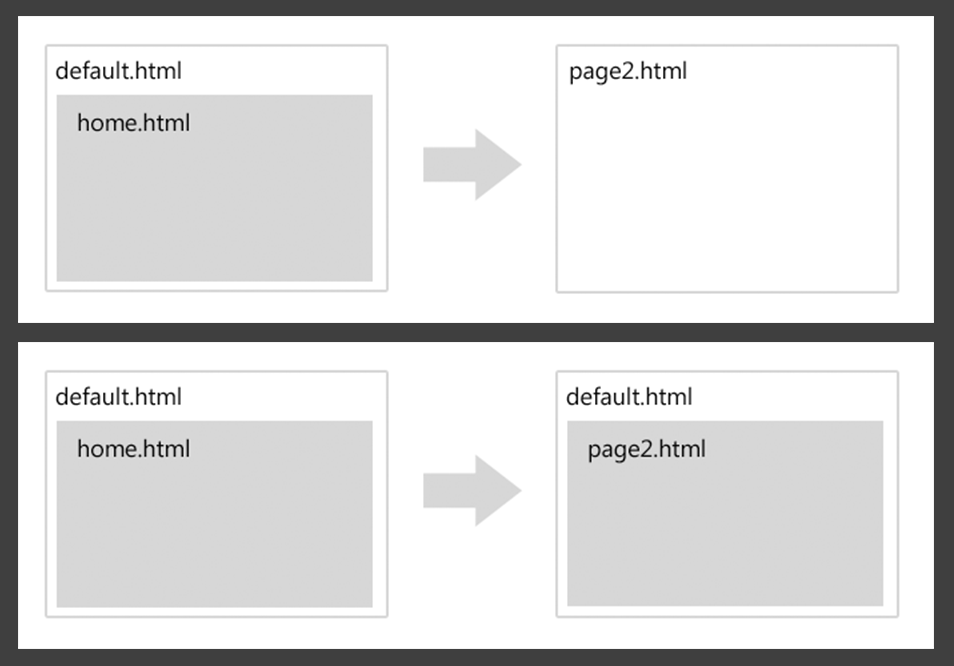
\includegraphics[width=0.6\textwidth]{Bilder/Abbildungen/single_page.png} 
	\caption[Die Single-Page-Navigation]{Oben: Die herkömmliche Navigation | Unten: die Single-Page-Navigation. \citep{MicrosoftSinglePage2013}}
	\label{fig:single-page}
\end{figure}

Es wird von Microsoft empfohlen, dass Windows-Store Apps, die mit \ac{html} und JavaScript erstellt werden, das single-page Navigationmodell verwenden. Die Navigation erfolgt nicht über Hyperlinks, sondern die verschiedenen Inhalte werden direkt in die Wrapper-Seite nachgeladen, ähnlich wie ein iframe. Abbildung \ref{fig:single-page} verdeutlicht das Single-Page-Navigation Konzept. Auf diese Weise gibt es keine sichtbare Unterbrechung beim Navigieren, d.h. es ist kein zwischenzeitlich weißer Bildschirm zu sehen. Außerdem erzielt man auf diese Weise eine bessere Performance und die App fühlt sich mehr \glqq app-like\grqq\ an. Die Rastervorlage verwendet das single-page Navigationsmodell \citep{MicrosoftSinglePage2013}. Abbildung \ref{fig:projektmappe} zeigt die Dateistruktur des Projektes. Anschließend wird erläutert, wofür die einzelnen Dateien verwendet werden.


\begin{figure}[h]
	\centering
	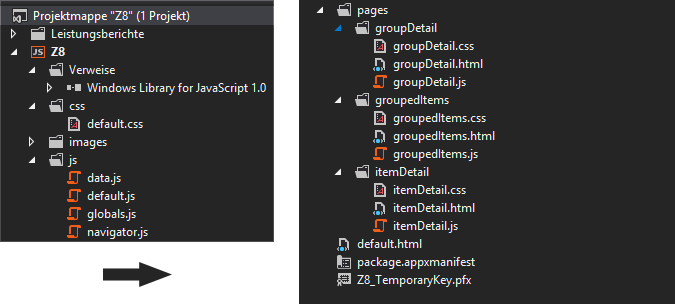
\includegraphics[width=\textwidth]{Bilder/Screenshots/app/projektmappe.png} 
	\caption{Die Projektstruktur in Visual Studio.}
	\label{fig:projektmappe}
\end{figure}

\subsubsection{HTML Dateien}
\label{subsubsec:htmldateien} 
Folgende \ac{html} Dateien sind bereits in der Raster-App Vorlage enthalten:
\begin{itemize}
	\item Die \textit{default.html} Datei wird als erstes geladen und enthält das \ac{html} für den Inhaltshost, dies ist die Seite, in welche die anderen Inhalte im Zuge der single-page Navigation herein geladen werden.
	\item Die \textit{groupedItems.html} Datei ist der Einstiegspunkt in die App (die Hubansicht).
	\item Die \textit{groupDetail.html} Datei zeigt alle Elemente eines Bereichs.
	\item Die \textit{itemDetail.html} Datei beinhaltet die Einzelansicht eines Elements.
\end{itemize}

\subsubsection{JavaScript Dateien}
\label{subsubsec:javascriptdateien} 
Folgende JavaScript Dateien sind bereits in der Raster-App Vorlage enthalten:
\begin{itemize}
	\item Die \textit{default.js} Datei legt fest, wie sich die App beim Start verhält.
	\item Die \textit{groupedItems.js}, \textit{groupDetail.js} und \textit{itemDetail.js} Dateien sind die JavaScript Dateien, welche das Verhalten für die gleichnamigen \ac{html} Dateien festlegen.
	\item Die \textit{navigator.js} Datei implementiert das hierarchische Navigationssystem sowie das single-page Navigationmodell.
	\item Die \textit{data.js} Datei stellt die benötigten Daten für den Rest der App bereit.
\end{itemize}

\subsubsection{CSS Dateien}
\label{subsubsec:cssdateien} 
Folgende CSS Dateien sind bereits in der Raster-App Vorlage enthalten:
\begin{itemize}
	\item Die \textit{default.css} Datei enthält die Styles für Inhaltshostseite sowie andere globale Styles.
	\item Die \textit{groupedItems.css}, \textit{groupDetail.css} und \textit{itemDetail.css} Dateien enthalten die Styles für die gleichnamigen \ac{html} Dateien.
\end{itemize}

Diese Vorlage wird nachfolgend angepasst und verändert, sodass sie die konzeptionierten Anforderungen erfüllt.

\subsection{Datenanbindung}
\label{subsec:datenanbindung}
Damit Nachrichten in der App angezeigt werden können, muss eine Datenverbindung zu ZEIT ONLINE hergestellt werden. Diese Verbindung ist nicht permanent aktiv. Beim Start der App werden zunächst die Basis-Daten eingelesen, anschließend werden nach Bedarf, z.B. wenn der User auf einen Artikel klickt, die benötigten Daten nachgeladen, indem eine weitere Anfrage abgesetzt wird. Zunächst wird erläutert, wie der Datenbestand von ZEIT ONLINE generiert wird. Anschließend wird darauf eingegangen, wie diese Daten in der App verfügbar gemacht werden.

\subsubsection{ZEIT ONLINE Datenbestand}
\label{subsubsec:zondatenbestand}
Es soll zunächst geklärt werden, wie sich der Inhalt der ZEIT ONLINE Website darstellt und wie er generiert wird. Die redaktionellen Inhalte werden fast ausschließlich über ein hauseigenes \ac{cms} erstellt und gepflegt. Das \ac{cms} generiert aus den Inhalten eine \ac{xml}-Struktur. Aus dem \ac{xml} wiederum wird anschließend mit Hilfe von \ac{xslt} das fertige \ac{html} erstellt.

Für ZEIGHT wird direkt das \ac{xml} verwendet, welches vom \ac{cms} generiert wird. Für die App werden zwei verschiedene Seitentypen der Webseite benötigt, um die gewünschten Informationen darzustellen, zum einen die verschiedenen \glqq Centerpages\grqq\ und zum anderen die Artikelansicht. Centerpages sind die Hauptseiten der jeweiligen Ressorts (z.B. die Hauptseite des Politik-Ressorts) sowie die Startseite mit den wichtigsten und aktuellsten Meldungen. Auf den Centerpages befinden sich die Teaserelemente für die verschiedenen Artikel. Die Teaserelemente bestehen meist aus einem Bild und einem kurzen, prägnanten Text, der erläutert, worum es in dem dahinter liegenden Artikel geht.\\

\begin{minipage}{\linewidth}
\begin{lstlisting}[language= XML,caption=Das XML eines Teaserelements, label={lst:knopfxml}]
<block href="http://xml.zeit.de/digital/internet/2013-08/fablab-open-hardware" year="2013" issue="34" ressort="Digital" author="Tilman Baumgärtel" contenttype="article" publication-date="" expires="" date-last-modified="2013-08-14T12:58:40+00:00" date-first-released="2013-08-14T09:57:43.627551+00:00" date-last-published="2013-08-14T12:59:39.691370+00:00" last-semantic-change="2013-08-14T09:56:40.185797+00:00">
	<supertitle>Open Hardware</supertitle>
	<title>Fab Labs, die Maschinen-Bibliotheken</title>
	<text>
		3-D-Drucker, CNC-Fräsen oder Lasercutter - mit solchen Maschinen sollen Bastler in Fab Labs experimentieren. Immer mehr solcher Werkstätten entstehen nun in aller Welt.
	</text>
	<description>
		3-D-Drucker, CNC-Fräsen oder Lasercutter - mit solchen Maschinen sollen Bastler in Fab Labs experimentieren. Immer mehr solcher Werkstätten entstehen nun in aller Welt.
	</description>
	<byline/>
	<image alt="MakerBot Replicator 2" align="left" title="MakerBot Replicator 2" base-id="http://xml.zeit.de/digital/internet/2013-08/makerbot-cebit-hannover/" type="jpg" publication-date="" expires="">
		<bu>
			Ein MakerBot Replicator 2 auf der diesjährigen Cebit in Hannover
		</bu>
		<copyright>© REUTERS/Fabrizio Bensch</copyright>
	</image>
</block>
\end{lstlisting}


\end{minipage}

Das \ac{xml} von einem Teaserelement ist in Listing \ref{lst:knopfxml} dargestellt. Es werden jedoch nicht alle Informationen aus dem \ac{xml} verwendet. Die verwendeten Informationen sind das \glqq date-first-released\grqq\ (Zeile 1), der \glqq title\grqq\ (Zeile 3), sowie die \glqq description\grqq\ (Zeile 7) und das \glqq image\grqq\ (Zeile 11). Das \ac{xml} für die Artikelansicht ist ähnlich aufgebaut, nur ist hier zusätzlich noch der Artikeltext in Form von Paragraphen-Tags (<p>) enthalten. Wie die Daten im Detail verarbeitet werden, wird im nächsten Abschnitt erläutert.

\subsubsection{Daten verfügbar machen}
\label{subsubsec:datenverfügbarmachen}
Die Daten, die in der App dargestellt werden sollen, werden grundsätzlich in zwei Schritten geladen. Wenn die App startet, werden zunächst alle benötigten Daten außer den eigentlichen Artikeln geladen. Der Artikelinhalt wird erst geladen, wenn der User ihn lesen will. Dies spart Zeit beim Starten der App, und der User hat somit ein flüssigeres App-Erlebnis. Der erste Schritt beim Einlesen und Verarbeiten der Daten geschieht in der \textit{data.js} Datei. Es werden alle Teaserelemente aller Ressorts letztendlich in einer  \textit{WinJS.Binding.List} gespeichert und für den weiteren Gebrauch verfügbar gemacht. Die \ac{winjs} ist eine JavaScript Bibliothek für Windows-Store Apps, die mit JavaScript erstellt werden. Sie enthält nützliche Funktionen z.B. für UI Steuerelemente oder sie hilft beim \ac{xhr}. Die Binding.List ist ebenfalls ein Teil dieser Bibliothek. Sie stellt Logik für die Datengruppierung bereit, genau in der Art und Weise, wie es für diese App sinnvoll ist. Falls mit dynamischen Daten gearbeitet, wird stellt sie z.B. Funktionen für die automatische Aktualisierung der Daten bereit. In Listing \ref{lst:bindinglst} ist die Initialisierung einer \textit{WinJS.Binding.List} dargestellt.

\begin{minipage}{\linewidth}
\begin{lstlisting}[language= Javascript,caption=Initialisierung der Binding-List., label={lst:bindinglst}]
var teaserElements = new WinJS.Binding.List();
\end{lstlisting}
\end{minipage}

Die Grundinformationen zu den einzelnen Ressorts wie der Name und die URL werden zunächst als normales JavaScript Array festgelegt. Einen Beispieleintrag aus dem Array zeigt Listing \ref{lst:ressortsarray}.

\begin{minipage}{\linewidth}
\begin{lstlisting}[language= Javascript,caption=Auszug aus dem Ressorts Array., label={lst:ressortsarray}]
ressorts = [
	{
	    key: "ressort01", url: 'http://xml.zeit.de/index',
	    title: 'Top Stories', subtitle: 'subtitle', updated: 'tbd',
	    backgroundImage: 'tbd', articleLink: "tdb",
	    acquireSyndication: acquireSyndication, dataPromise: null
    }
]
\end{lstlisting}
\end{minipage}

Anschließend wird eine weitere Funktion von \ac{winjs} verwendet, die \textit{WinJS.Promises}. Mit Promises kann mit asynchronen Prozessen und Datenquellen umgegangen werden. Hier werden für alle Ressorts \ac{xhr}s gestartet, an die im Ressorts-Array angegebene URLs. Alle \ac{xhr}s werden ebenfalls in einem Array gespeichert und erst wenn alle Promises vorhanden sind (alle URL waren erreichbar), wird die Datenverarbeitung fortgesetzt. \\
Mit den vorhandenen und validen \ac{xhr} Responses können anschließend alle Teaserelemente in einer Schleife durchlaufen, das \ac{xml} geparst und so die nötigen Informationen für die App verfügbar gemacht werden. Listing \ref{lst:xmlparsing} zeigt wie der Titel (Zeile 10), der Teasertext (Zeile 13) und der Bildpfad (Zeilen 15-22) aus dem \ac{xml} gewonnen werden. Am Ende der Funktion werden die Daten in die in Listing \ref{lst:bindinglst} erstellte \textit{WinJS.Binding.List} geschrieben (Zeilen 24-28). Die dargestellte Funktion ist nicht vollständig und wurde aus Übersichtlichkeitsaspekten und Relevanzgesichtspunkten verkürzt dargestellt.

\begin{minipage}{\linewidth}
\begin{lstlisting}[language= Javascript,caption=Parsen und Speichern der Daten., label={lst:xmlparsing}]
function getItemsFromXml(ressortXML, teaserElements, ressort) {
    var teasers = ressortXML.querySelectorAll("region[area='lead'] container > block:first-child");
    // Process each ressort teaser.
    for (var teaserIndex = 0; teaserIndex < teasers.length; teaserIndex++) {
        var teaser = teasers[teaserIndex];

       //only articles with an image are alllowed
        if (teaser.getAttribute("contenttype") == "article" && teaser.querySelector("image") !== null) {
            // Get the title
            var teaserTitle = teaser.querySelector("title").textContent;
        
            // Process the content so that it displays nicely.
            var staticContent = toStaticHTML(teaser.querySelector("description").textContent);

            //Get and build the image path
            var teaserImageEl = teaser.querySelector("image");
            var imageBasePath = teaserImageEl.getAttribute("base-id");
            var splitImagePath = imageBasePath.split('/');
            var imageNameSmall = splitImagePath[splitImagePath.length - 2] + "-220x124.jpg";
            var imageNameBig = splitImagePath[splitImagePath.length - 2] + "-540x304.jpg";
            var imagePathSmall = imageBasePath + imageNameSmall;
            var imagePathBig = imageBasePath + imageNameBig;
            
            // Store the teaser element info we care about in the array.
            teaserElements.push({
                group: ressort, key: ressort.title, title: teaserTitle,
                backgroundImage: imagePathBig, teaserText: staticContent
            });
        }
    }
}
\end{lstlisting}   
\end{minipage}

Sobald die Daten in der \textit{WinJS.Binding.List} gespeichert sind, können sie vom Rest der App weiterverwendet und grafisch aufbereitet werden. Es wurden bisher noch keine Artikelinhalte geladen, dies geschieht erst dann, wenn der User auf einen Artikel klickt.

\subsection{Darstellung der Daten}
\label{subsec:darstellungderdaten}
In diesem Abschnitt wird darauf eingegangen, wie die zuvor verarbeiteten und gespeicherten Daten für eine ansprechende Darstellung in der App aufbereitet werden.

\subsubsection{Die Hubansicht}
\label{subsubsec:hubansicht}
Wenn die App startet, befindet sich der User in der Hubansicht. Hier werden ihm für alle Haupt-Ressorts die ersten sechs Artikel angezeigt, in der Reihenfolge wie sie auch auf der Webseite zu finden sind (siehe Abbildung \ref{fig:hubressortübersicht}).

Zu der Hubansicht gehören eine \ac{html} Datei, in welcher das Markup festgelegt ist, eine CSS Datei, die das Layout der Seite bestimmt und eine JavaScript Datei, in der das Verhalten (die Logik) der Hubseite programmiert wird. 

\begin{figure}[h]
	\centering
	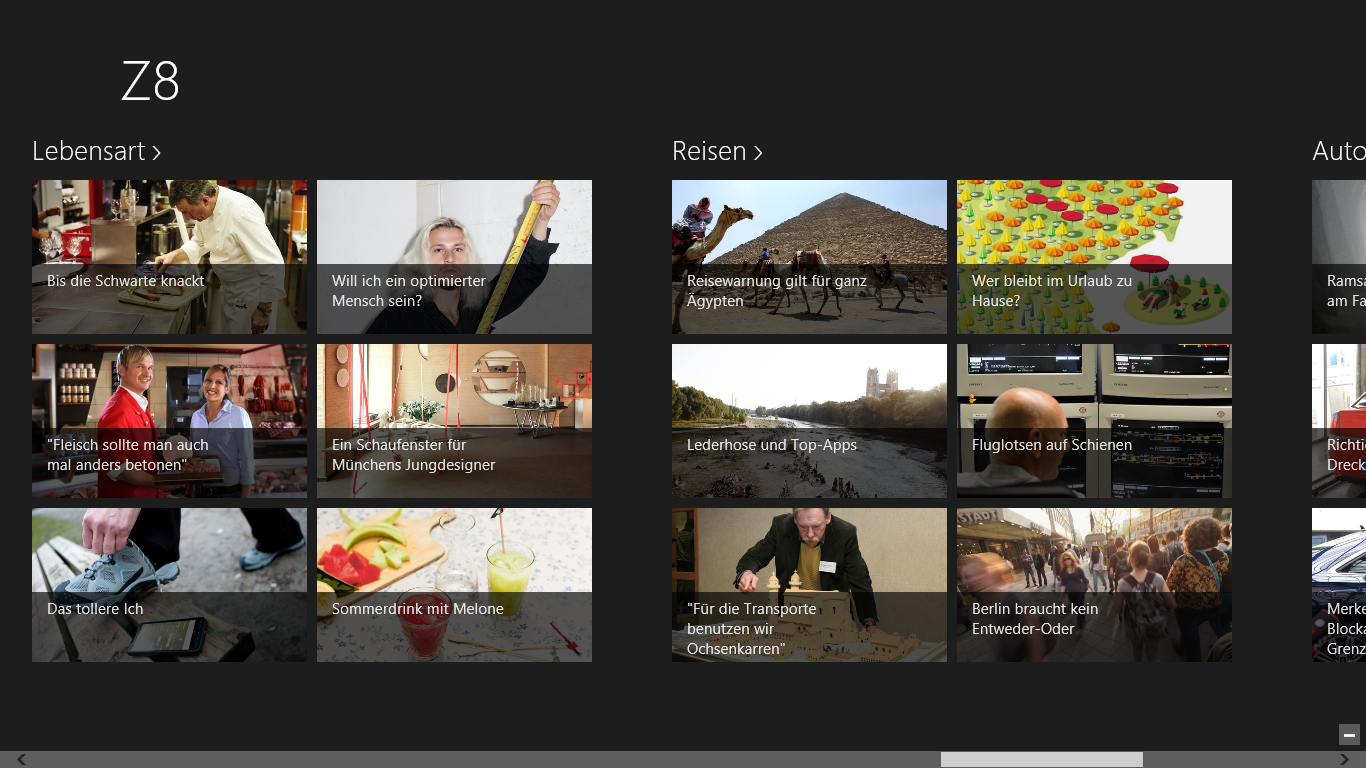
\includegraphics[width=\textwidth]{Bilder/Screenshots/app/reise_aegypten_2gmit.png} 
	\caption{Die Hubansicht.}
	\label{fig:hubressortübersicht}
\end{figure}

Um die Daten aus der \textit{WinJS.Binding.List} auf der Hubseite anzeigen zu können, sind einige Schritte notwendig. Zunächst soll der Aufbau der \ac{html} Datei erläutert werden. Listing \ref{lst:hubmarkup} zeigt einen Ausschnitt aus der \textit{groupedItems.html} Datei. Im oberen Teil befindet sich ein Template mit der Klasse \textit{itemtemplate}, welches auf jedes einzelne Element der Hubansicht angewandt wird. Das Besondere an diesem Template ist, dass es ein \textit{data-win-control} Attribut mit dem Wert \glqq WinJS.Binding.Template\grqq\ besitzt. Es akzeptiert Daten aus einer \textit{WinJS.Binding.List}, wie sie in der Rohdatenverarbeitung genutzt wurde. Im unteren Teil ab Zeile 10 steht der Container für den eigentlichen Inhalt. Dieses Objekt besitzt ein \textit{data-win-control} Attribut mit dem Wert \glqq WinJS.ListView\grqq. Eine \textit{WinJS.ListView} stellt Elemente in anpassbaren Listen oder Rastern dar. 

\begin{minipage}{\linewidth}
\begin{lstlisting}[language= XML,caption=Die wichtigsten Markupelemente der Hubansicht., label={lst:hubmarkup}]
<div class="itemtemplate" data-win-control="WinJS.Binding.Template">
    <div class="item">
        <img class="item-image" src="#" data-win-bind="src: backgroundImage; alt: title" />
        <div class="item-overlay">
            <h4 class="item-title" data-win-bind="textContent: title"></h4>
        </div>
    </div>
</div>

<section aria-label="Main content" role="main">
    <div class="groupeditemslist win-selectionstylefilled" aria-label="List of groups" data-win-control="WinJS.UI.ListView" data-win-options="{selectionMode: 'none'}"></div>
</section>
\end{lstlisting}   
\end{minipage}

Der Rest passiert in der \textit{groupedItems.js} Datei. Die \textit{groupedItems.js} besitzt eine \textit{ready()} Methode. Diese wird jedesmal aufgerufen, wenn der User zur Hubansicht wechselt oder die Hubansicht wiederhergestellt wird. Um die Daten in der \textit{WinJs.ListView} zu hinterlegen wird, als erstes die \textit{WinJS.ListView} in einer Variable gespeichert und anschließend das gewünschte Template bei der ListView registriert (siehe Listing \ref{lst:getitemtemplate}). 

\begin{minipage}{\linewidth}
\begin{lstlisting}[language= Javascript,caption=Template bei der Listview registrieren., label={lst:getitemtemplate}]
var listView = element.querySelector(".groupeditemslist").winControl;
listView.itemTemplate = element.querySelector(".itemtemplate");
\end{lstlisting}   
\end{minipage}

Anschließend wird die \textit{initializeLayout} Funktion aufgerufen. Hier wird am Anfang eine entscheidende Operation ausgeführt. In der \textit{WinJS.Binding.List} sind bisher alle Teaserelemente aus allen Ressorts enthalten, für die Hubansicht sind aber nur sechs Elemente pro Ressort gewünscht. Deswegen wird eine Funktion \textit{getClippedList()} in der \textit{data.js} Datei aufgerufen, welche die ersten sechs Elemente jedes Ressorts zurück liefert. Damit die Elemente wie gewünscht angezeigt werden können, muss noch die \textit{dataSource} der \textit{WinJS.ListView} gesetzt werden, ebenso wie das Raster-Layout (siehe Listing \ref{lst:setdatasource}). Nach diesem Schritt werden die ersten sechs Elemente jedes Ressorts wie in Abbildung \ref{fig:hubressortübersicht} angezeigt.

\begin{minipage}{\linewidth}
\begin{lstlisting}[language= Javascript,caption=Setzen der Datenquelle und des Layouts., label={lst:setdatasource}]
listView.itemDataSource = groupedItemsHub.dataSource;
listView.layout = new ui.GridLayout({ groupHeaderPosition: "top" });
\end{lstlisting}   
\end{minipage}

\subsubsection{Die Ressortansicht}
\label{subsubsec:ressortansicht}
Die Ressortansicht, die zweite Detailstufe zeigt alle Elemente eines Ressorts (siehe Abbildung \ref{fig:einzelressortübersicht}). Der User gelangt hierhin, wenn er in der Hubansicht auf den Ressortnamen im Headerbereich klickt. 

\begin{figure}[h]
	\centering
	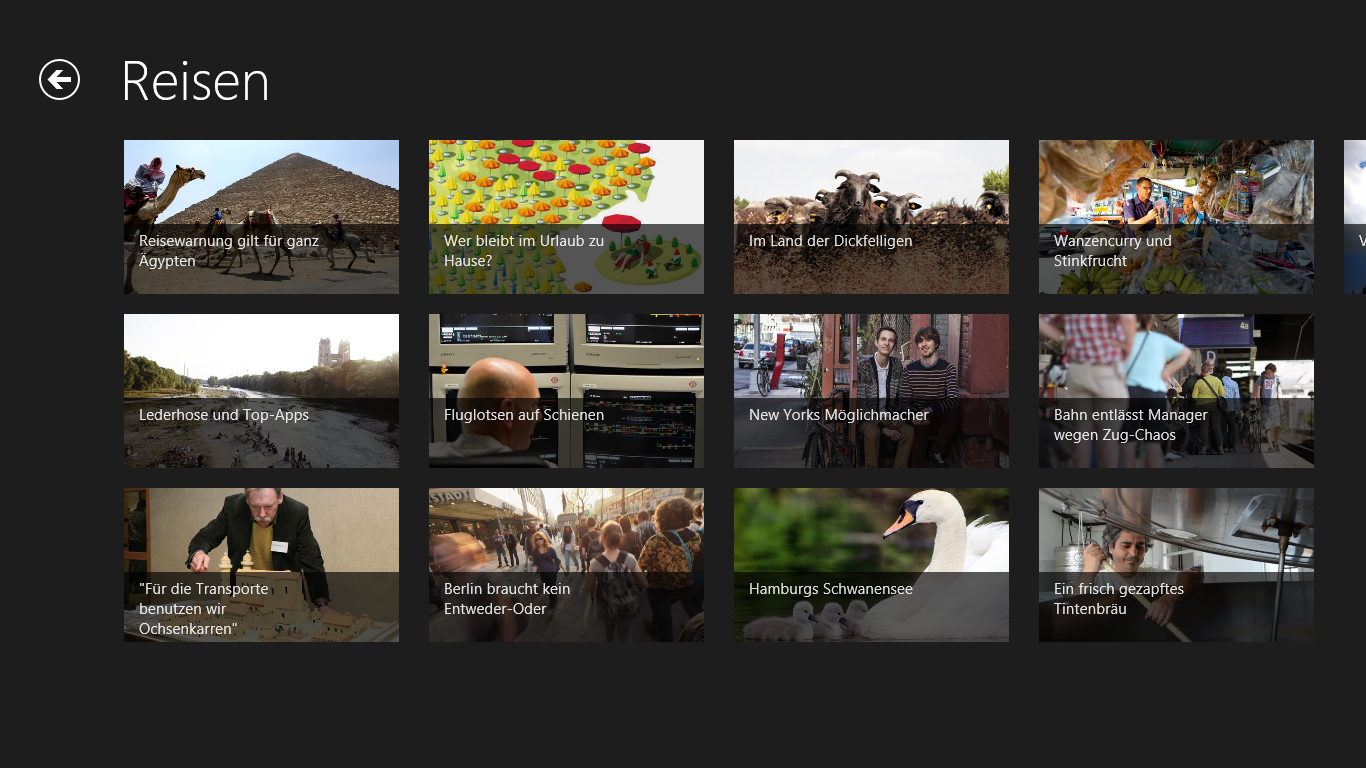
\includegraphics[width=\textwidth]{Bilder/Screenshots/app/reise_aegypten_3gdmit.png} 
	\caption[Die Einzelressortübersicht]{Die Einzelressortübersicht (hier das Reisen-Ressort).}
	\label{fig:einzelressortübersicht}
\end{figure}

Die Programmlogik funktioniert analog zur Hubansicht. Es werden die gleichen Mechanismen zur Darstellung des Raster-Musters benutzt. Auch die zu dieser Ansicht gehörende \ac{html} und JavaScript Dateien ähneln denen von der Hubansicht sehr. Ein wesentlicher Unterschied besteht darin, dass im Gegensatz zu Hubansicht nicht die Funktion \textit{getClippedList()}, sondern stattdessen die Funktion \textit{getItemsFromGroup()} aufgerufen wird. Sie gibt alle Elemente der übergebenen Gruppe zurück. Diese können nun mit einem \textit{itemTemplate} und einer \textit{WinJS.ListView} dargestellt werden. 

\subsubsection{Die Artikelansicht}
\label{subsubsec:artikelansicht}
Die Artikelansicht ist die letzte Detailstufe. Sie zeigt den eigentlichen Artikelinhalt (siehe Abbildung \ref{fig:artikelansicht}). Dargestellt werden das Ressort, der Titel, der Teasertext, das Aufmacherbild in groß, die Bildunterschrift, das Copyright für das Bild, der Artikeltext, die Quelle des Artikels (z.B. ZEIT ONLINE oder dpa), der Autor sowie das Erstellungsdatum. Die Artikeldarstellung funktioniert etwas anders als die Hub- und der Ressortdarstellung. Es wird kein Template verwendet, stattdessen wird das \ac{html} mit Hilfe von JavaScript befüllt. In der \textit{ready()} Funktion der \textit{itemDetail.js} Datei werden zunächst die bereits vorhandenen Informationen in das \ac{html} eingefügt.

\begin{figure}[h]
	\centering
	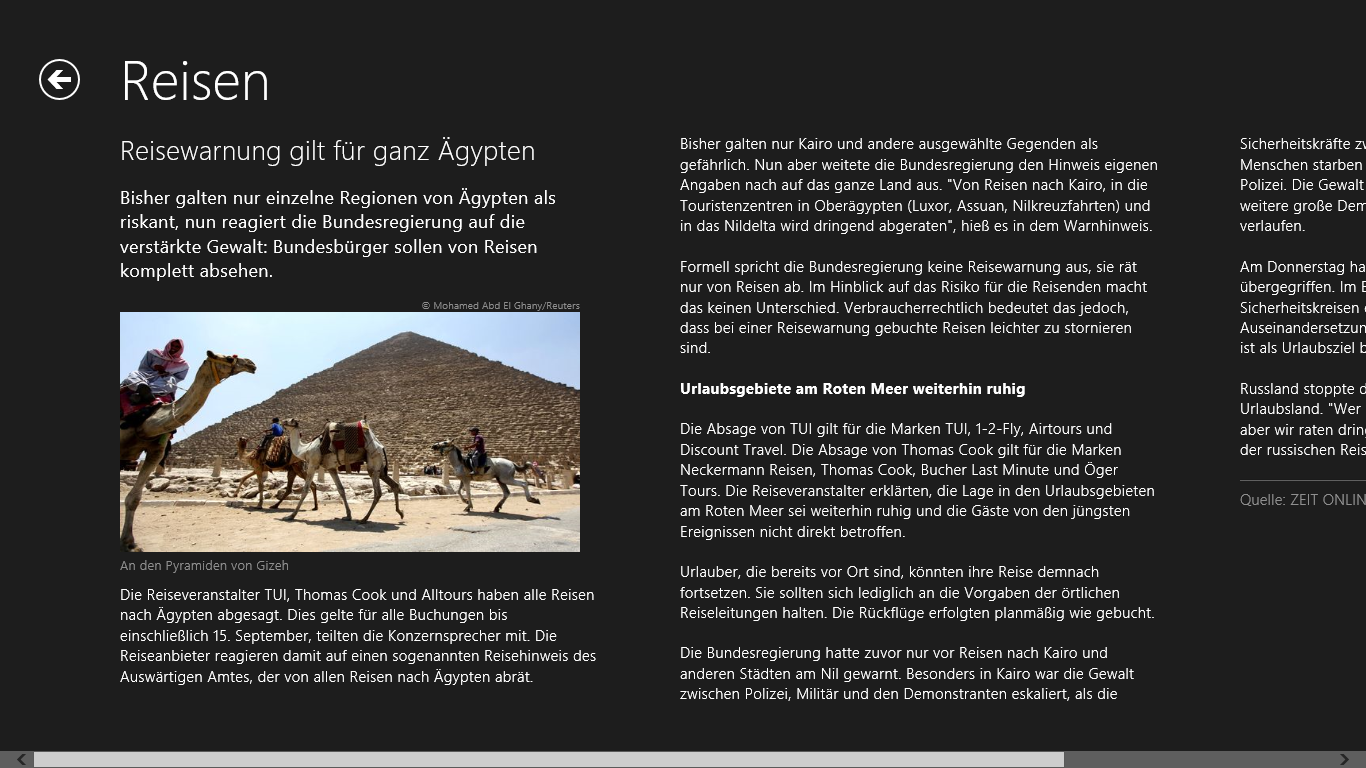
\includegraphics[width=\textwidth]{Bilder/Screenshots/app/reise_aegypten_4d.png} 
	\caption{Die Artikelansicht.}
	\label{fig:artikelansicht}
\end{figure}

Listing \ref{lst:artikelinfos} zeigt das Einfügen von Titel, Teasertext und  dem Bild. Anschließend fehlt noch der Artikeltext, die Quelle und der Autor. Um diese Daten zu bekommen und zu speichern, ist ein weiterer \ac{xhr} nötig. Der \ac{xhr} wird mit der Artikel-URL aufgerufen, die in jedem Teaserelement gespeichert ist. Auf diese Weise bekommt man das \ac{xml} der Artikel, wie es auch von der Webseite verwendet wird. 

\begin{minipage}{\linewidth}
\begin{lstlisting}[language= Javascript,caption=Das Einfügen von Titel sowie Teasertext und Bild., label={lst:artikelinfos}]
element.querySelector("article .item-title").textContent = item.title;
element.querySelector("article .item-subtitle").innerHTML= item.teaserText;
element.querySelector("article .item-image").src = item.backgroundImage;
\end{lstlisting}   
\end{minipage}

Beim Parsen des Artikel-\ac{xml}s müssen folgende drei Sachverhalte besonders beachtet werden. Die Absätze des Artikels liegen in Paragraphen-Tags (<p></p>) vor. Es kann vorkommen, dass außer dem reinen Text, zusätzlich noch Infoboxen im Artikel vorhanden sind. Der zweite Besonderheit ist die, dass Nachrichten vom Mikroblogging Dienst Twitter eingebunden werden können. Diese Abschnitte arbeiten ebenfalls mit Paragraphen-Tags. Da Infoboxen und Twitternachrichten sich inhaltlich nicht direkt in den Artikeltext eingliedern, müssen diese Abschnitte vorher herausgefiltert werden. Des Weiteren sind in den meisten Artikeln auf der ZEIT ONLINE Webseite Hyperlinks auf andere Artikel oder auf andere Webseiten vorhanden. Diese sind genau wie Infoboxen und Twitternachrichten unerwünscht, da sie, wenn sie vom User aufgerufen werden, außerhalb der aktuellen App im Browser geöffnet würden. Dies unterbricht und stört das App-Erlebnis. Es muss dementsprechend darauf geachtet werden, dass nur der reine Artikeltext als Artikel gespeichert wird. Listing \ref{lst:artikelabsätze} verdeutlicht, wie dies umgesetzt wird. In Zeile 3 werden die Infoboxen und die Twitternachrichten herausgefiltert und in den Zeilen 8-13 werden die \textit{<a></a>} Tags mit Hilfe regulärer Ausdrücke gelöscht. Sobald der Artikel komplett geladen ist, wird er analog zu Listing \ref{lst:artikelinfos} in das \ac{html} Markup eingefügt.

\begin{minipage}{\linewidth}
\begin{lstlisting}[language= Javascript,caption=Vermeidung von Infoboxen \, Twitternachrichten und Hyperlinks in den Artikeln., label={lst:artikelabsätze}]
for (var n = 0; n < paragraphs.length; n++) {
    //exclude info box and tweets paragraphs
    if (paragraphs[n].parentNode.parentNode.parentNode.parentNode.nodeName != "infobox" && paragraphs[n].parentNode.getAttribute("class") != "twitter-tweet"){
        var xmlText = new XMLSerializer().serializeToString(paragraphs[n]);
        if (paragraphs[n].querySelector("a") != null) {
            var numberOfLinks = paragraphs[n].querySelectorAll("a").length;
            //remove hyperlinks
            for (var i = 0; i < numberOfLinks; i++) {
                var rx = new RegExp("<a[^<>]+>", "i");
                xmlText = xmlText.replace(rx, "");
                rx = new RegExp("</a>", "i");
                xmlText = xmlText.replace(rx, "");
            }
        }
        textContent = textContent + xmlText;
    }
}
\end{lstlisting}   
\end{minipage}

\subsection{Features}
\label{subsec:features}
Im Folgenden werden die Features der ZEIGHT App erläutert. Es handelt sich hierbei zum einen um die Einstellungen, die der User über die untere Menüleiste vornehmen kann, und zum anderen um das \glqq Semantic Zoom\grqq\ Feature.

\subsubsection{Artikeltitel ausblenden}
\label{subsubsec:artikeltitelausblenden}
Ein Hauptfeature der App ist es, dass in der Hubansicht und in der Ressortansicht die Artikeltitel ausgeblendet werden können und der User so nur noch eine Bilderwand vor sich hat. So kann er die Nachrichtenlage rein visuell erleben, und erst wenn er auf einen Artikel klickt, bekommt er im Artikel den Titel und Artikelinhalt zu sehen. Diese Funktion wird über eine Menüleiste am unteren Bildrand implementiert (siehe Abbildung \ref{fig:menubartitletoggle}). Um eine solche Menüleiste zu erzeugen, genügt ein \textit{<div>} Container in der \textit{default.html} Datei mit einem \textit{data-win-control} Attribut, das den Wert \glqq WinJS.UI.AppBar\grqq\ bekommt. In diesem Element können anschließend \textit{<button>} Elemente angelegt werden. Diese sind später die sichtbaren Schaltflächen, wenn die Menüleiste aufgerufen wird.

\begin{figure}[h]
	\centering
	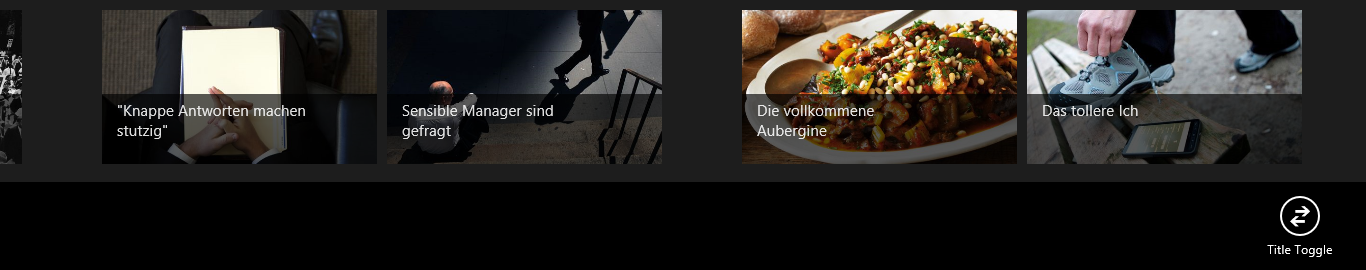
\includegraphics[width=\textwidth]{Bilder/Screenshots/app/title_toggle_menu_bar.png} 
	\caption{Die untere Menüleiste mit der Funktion zum Artikeltitel ausschalten.}
	\label{fig:menubartitletoggle}
\end{figure}

In der Initialisierungsphase der App wird in der \textit{default.js} Datei der Click-Handler für den Button registriert. Hier wird die Funktion angegeben, die aufgerufen werden soll, wenn der Button geklickt wird. In diesem Fall wird die Funktion \textit{titleToggle()} in der \textit{globals.js} Datei aufgerufen. In der \textit{globals.js} Datei befinden sich Variablen und Funktionen, die von mehreren Ansichten benutzt werden und deswegen global verfügbar sein sollen. Die \textit{titleToggle()} Funktion ist schließlich verantwortlich für das Ausblenden der Artikeltitel.

Die Funktion sammelt dazu alle Elemente mit der Klasse \textit{item-overlay} in einem Array und setzt anschließend für alle gefundenen Elemente die CSS Eigenschft \textit{display} auf \glqq none\grqq\ . Das Resultat ist in Abbildung \ref{fig:ressortohnetitel} zu sehen.

\begin{figure}[h]
	\centering
	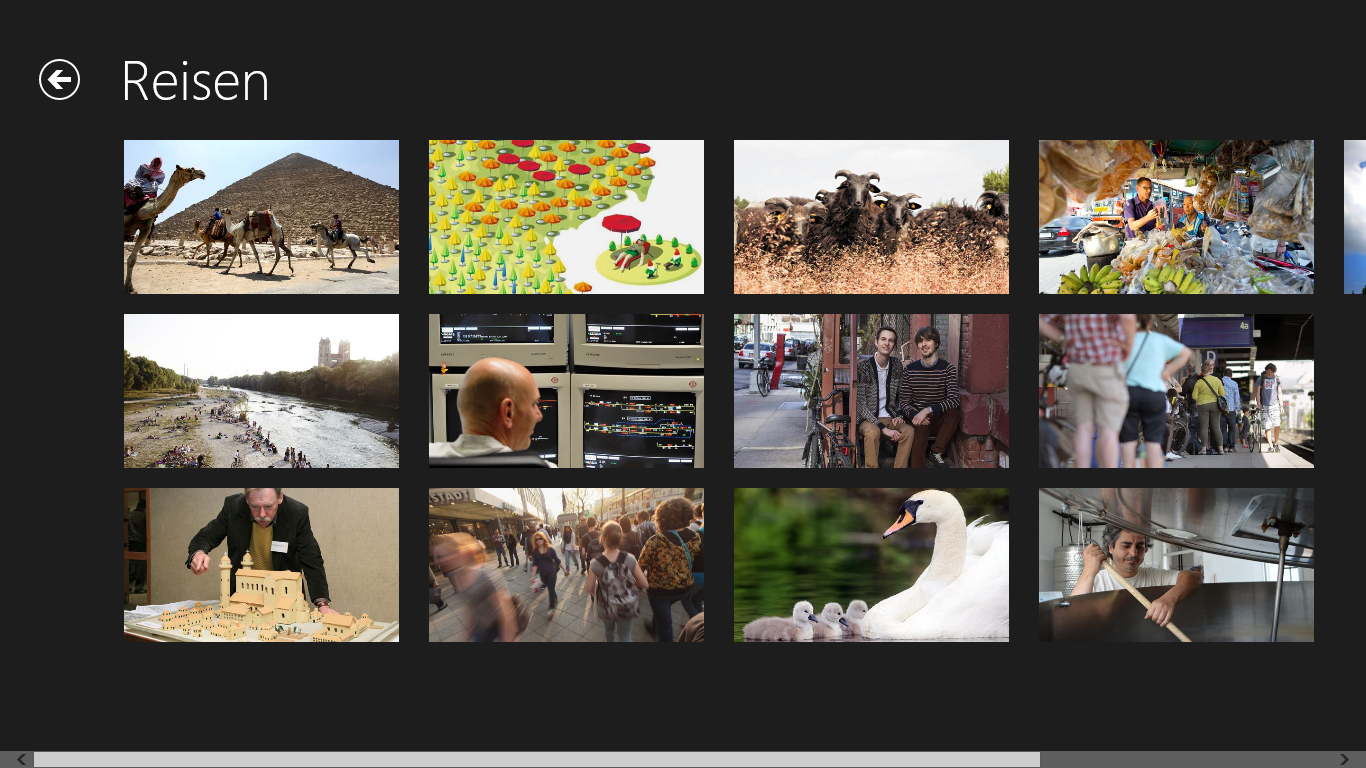
\includegraphics[width=\textwidth]{Bilder/Screenshots/app/reise_aegypten_3gdohne.png} 
	\caption{Das Reisen-Ressort ohne Artikeltitel.}
	\label{fig:ressortohnetitel}
\end{figure}

\subsubsection{Schriftgröße verändern}
\label{subsubsec:schriftgroesseveraendern}
In der Artikelansicht hat der User die Möglichkeit, die Schriftgröße anzupassen. Es sind jeweils zwei Stufen größer als auch zwei Stufen kleiner als die normale Größe möglich. Der  Ansatz ist grundsätzlich genau so wie bei der \glqq Titel-Ausblenden\grqq\ Funktionalität. Zunächst wird ein Button in der unteren Menüleiste angelegt. Es wäre auch möglich, zwei Buttons zu erstellen, einen für größer und einen für kleiner. Um weitere  Entwicklungsmöglichkeiten der \ac{winjs}-Bibliothek auszunutzen, gibt es in der App nur einen Button in der Menüleiste. Wird dieser geklickt, erscheint noch ein weiteres Menü, ein sogenanntes \textit{Flyout-Menü}. In diesem sind schließlich die Schaltflächen für \glqq Schrift größer\grqq\ , \glqq Schrift kleiner\grqq\ und für \glqq Schriftgröße zurücksetzen\grqq\ hinterlegt. Ist die Schriftgröße z.B. auf der größten Stufe eingestellt, wird im Menü der \glqq Größer Button\grqq nicht mehr dargestellt. Abbildung \ref{fig:fontsizemenü} zeigt die verschiedenen Stati, die das Schriftgrößenmenü haben kann.

\begin{figure}[h]
	\centering
	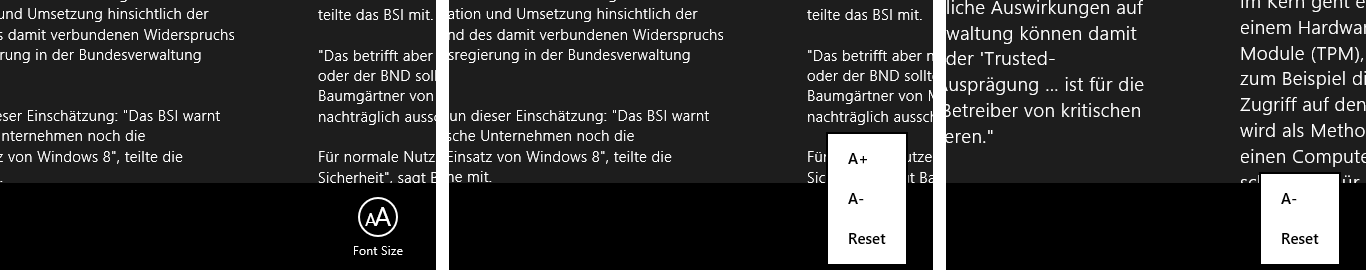
\includegraphics[width=\textwidth]{Bilder/Screenshots/app/font_size_menu_kompakt.png} 
	\caption[Die Schriftgröße-Buttons]{Links: Schriftgröße Button im unteren Menü | Mitte: Das Flyout-Menü mit allen Schaltflächen. |Rechts: Das Flyout-Menü beim Aufruf wenn der größte Wert eingestellt ist.}
	\label{fig:fontsizemenü}
\end{figure} 

\subsubsection{Semantic Zoom}
\label{subsubsec:semanticzoom}
Das \glqq Semantic Zoom\grqq\ Feature wird eingesetzt, wenn es in der Hubansicht sehr viele Bereiche gibt. Es soll dem User ermöglichen ohne langes Scrollen, zu den verschiedenen Bereichen in der Hubansicht zu springen. Beim Aufruf des \glqq Semantic Zooms\grqq\ wird eine weitere Ebene über die Hubansicht gelegt. Typischer Weise werden in dieser Ebene die verschiedenen Bereiche ohne inhaltliche Elemente angezeigt. Bei ZEIGHT werden hier alle Ressorts mit dem jeweiligen Ressortnamen und einem zufälligen Bild aus dem Ressort angezeigt (siehe Abbildung \ref{fig:semanticzoom}). Diese Ansicht ist ebenfalls horizontal scrollbar, im direkten Vergleich zur Hubansicht jedoch viel kompakter und übersichtlicher. Klickt der User z.B. auf das Reisen-Ressort, wird wieder zurück zur Hubansicht \glqq gezoomt\grqq. Der User hätte dann die Ansicht, wie sie Abbildung \ref{fig:hubressortübersicht} auf Seite \pageref{fig:hubressortübersicht} zeigt. Damit findet in beide Richtungen ein kontextsensitives Zoomen statt. Je nach dem wo sich der User in der Hubansicht befindet bzw. auf welches Ressort der User in der \glqq Semantic Zoom\grqq\ Ebene klickt, wird an die entsprechende Stelle raus- bzw. reingezoomt.  

\begin{figure}[h]
	\centering
	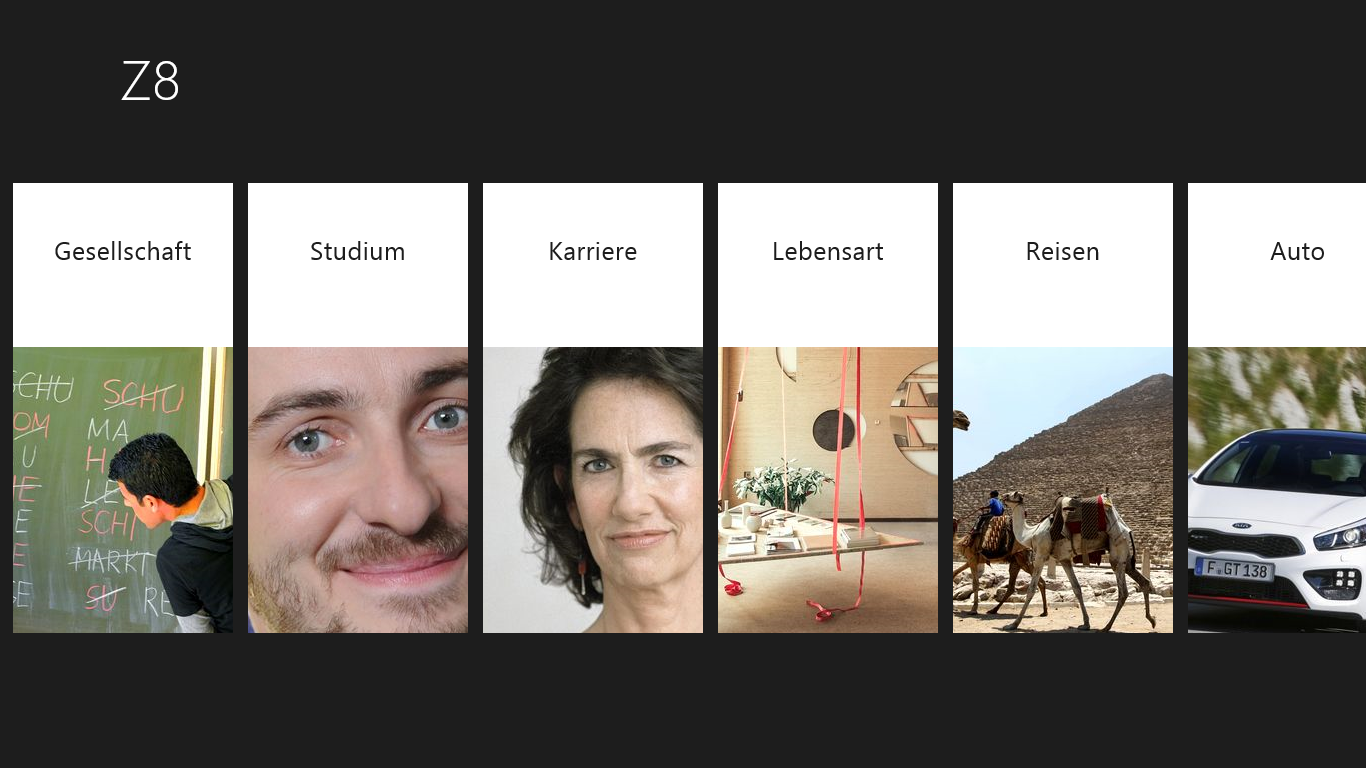
\includegraphics[width=\textwidth]{Bilder/Screenshots/app/reise_aegypten_1zoom.png} 
	\caption[Die Semantic Zoom Ansicht]{Die \glqq Semantic Zoom\grqq\ Ansicht.}
	\label{fig:semanticzoom}
\end{figure}  

Da der semantic Zoom von der Hubansicht aus aufgerufen wird und mit ihr interagiert, ist er dementsprechend in der \textit{groupedItems.html} und in der\textit{groupedItems.js} implementiert. Genau wie für die Hubansicht gibt es auch für den semantic Zoom ein Template für die einzelnen Elemente. Damit eine Interaktion zwischen der Hubansicht und dem semantic Zoom stattfinden kann, wird ein Wrapper \textit{div} Element um die \textit{WinJS.ListView} der Hubansicht und die \textit{WinJS.ListView} der \glqq Semantic Zoom\grqq\ Ebene gezogen. Listing \ref{lst:semanticzoomwrapper} zeigt, wie der Wrapper eingebunden ist. Das \textit{div} Element besitzt ein \textit{data-win-control} Attribut mit dem Wert \glqq WinJS.UI.SemanticZoom\grqq. Des Weiteren kann der \textit{zoomFactor} und der initiale Zoomstatus festgelegt werden. Bei der ZEIGHT App steht dieser Zoomstatus initial auf \glqq false\grqq, da der User die Hubansicht als Einstiegspunkt in die App haben soll und nicht die \glqq Semantic Zoom\grqq\ Ansicht.

\begin{minipage}{\linewidth}
\begin{lstlisting}[language= XML,caption=Der Semantic Zoom Wrapper., label={lst:semanticzoomwrapper}]
<div class="semanticZoom" data-win-control="WinJS.UI.SemanticZoom" data-win-options="{ zoomFactor: 0.5, initiallyZoomedOut: false }" style="height: 100%">
    <div class="groupeditemslist win-selectionstylefilled" aria-label="List of groups" data-win-control="WinJS.UI.ListView" data-win-options="{selectionMode: 'none'}"></div>
    <div class="groupeditemslistZoomOut groupeditemslist" aria-label="List of groups" data-win-control="WinJS.UI.ListView" data-win-options="{selectionMode: 'none'}"></div>
</div>
\end{lstlisting}   
\end{minipage}

\subsection{Entwicklungschronologie}
\label{subsec:entwicklungschronologie}
Hier soll beschrieben werden, wie der Entwicklungsprozess von ZEIGHT abgelaufen ist. Nachdem die Idee für die App formuliert war, hat sich der Verfasser zunächst mit der Windows 8 App Entwicklung im Allgemeinen vertraut gemacht, da bis zu diesem Zeitpunkt keinerlei Windows 8 spezifische Entwicklungskenntnisse vorhanden waren. Es wurden einige Beispiele ausprobiert, um ein Gefühl für die Entwicklungsumgebung zu bekommen. Der Workflow zwischen Visual Studio und Blend war am Anfang noch etwas gewöhnungsbedürftig. Anschließend wurde ein erster Prototyp erstellt. Hier fanden noch keine Überlegungen zum Navigationssystem oder zur Usability statt. Am Anfang gab es zunächst nur das nur das Ziel, die ZEIT ONLINE Daten in irgendeiner Weise in die App zu übernehmen und sie dort darzustellen. In einer der ersten Versionen der App wurden z.B. nur die Artikeltitel der Homepage angezeigt. Nachdem die Datenanbindung umgesetzt war, konnte mit dem Entwickeln der richtigen App begonnen werden.

Es wurde zunächst viel recherchiert, zu nennen sind hier insbesondere die Microsoft Richtlinien und Styleguides, um herauszufinden, wie aus Microsoft Sichtweise eine Nachrichten-App auszusehen hat. Dabei war immer wieder die Rede von der Rastervorlage, die sich für solche Zwecke eignen solle. Diese Grundvorlage wurde schließlich für die App ausgewählt. Da die Rastervorlage keine triviale Vorlage ist, musste einige Zeit investiert werden, um alle Vorgänge und Dateien der Vorlage richtig ein- und zuordnen zu können. 

Eines der ersten größeren Probleme war die Dezimierung der Daten für die Hubansicht. Hier musste die Funktion \textit{getClippedList} entwickelt werden (wie in Abschnitt \ref{subsubsec:hubansicht} beschrieben). Des weiteren wurde in dieser Phase das CSS für Hubansicht und die Ressortübersicht angepasst. Gerade bei der Ressortansicht musste einiges an der Vorlage verändert werden.

Danach wurden die Menüleisten hinzugefügt  und die \textit{titleToggle} zum Ausschalten der Artikeltitel programmiert. Da bisher noch keine Versionierung der App vorhanden war, wurde zu diesem Zeitpunkt ein GitHub Repository angelegt\footnote{Link zum GitHub Repository: https://github.com/mohdr0w/Z8} und die App unter Versionskontrolle gestellt. 

Anschließend wurde die Artikelansicht gestaltet und dabei die Bildunterschriften und die Copyrights positioniert. Leider kann bei Entwicklung mit HTML5/JavaScript nicht direkt auf die Scrollposition der Hubansicht zugegriffen werden. Deswegen landete der User beim Wechseln in die Hubansicht immer wieder ganz am Anfang. Da dies nicht zufriedenstellend war, wurde die Funktionalität manuell nachgerüstet, indem der Index des ersten sichtbaren Elements global gespeichert wird und beim Aufrufen der Hubansicht wieder gesetzt wird. Eine weitere manuell nachgerüstete Funktionalität ist der \textit{loading Ring} beim Laden der App. Hierfür wird auf die Events der \textit{WinJS.ListView} zurückgegriffen und die Animation ausgeblendet, sobald die ListView geladen ist.

Anschließend wurde die Verarbeitung der Artikel vereinfacht. Am Anfang wurden die \textit{<p></p>} Elemente erst \glqq auseinander genommen\grqq\ und anschließend wieder zusammengesetzt. Da das \ac{xml} der Artikel aber schon valides \ac{html} enthält, konnte einfach der ganze Text samt Zwischenüberschriften übernommen werden. Was noch herausgefiltert werden musste, sind Infoboxen und Twitternachrichten, die in den Artikeln eingebaut sein können. Als nächstes wurde das \textit{Semantic Zoom} Feature sowie die Funktionalität zur Veränderung der Schriftgröße implementiert.   

Zu diesem Zeitpunkt hat es eine kleine strukturelle Ergänzung im \ac{xml} von ZEIT ONLINE gegeben. Die Teaserelemente haben nun jeweils ein Attribut \textit{contenttype}. Da in der App nur Artikel dargestellt werden sollen, kann auf diese Weise bequem nach \glqq contenttype = article\grqq gefiltert werden. Dies ist eine große Vereinfachung, denn zuvor wurden nach dem Negativ-Prinzip recht aufwändig alle anderen Typen wie z.B. Videos, Blogartikel oder Quizze ausgeschlossen.  

Gegen Ende der Entwicklung wurde noch der Snapped Modus der App unterbunden. Normalerweise können Windows 8 Apps außer dem Vollbildmodus auch noch im Snapped-Modus ausgeführt werden. Dabei wird der Bildschirm vertikal getrennt, und es können zwei Apps im Verhältnis 70:30 nebeneinander dargestellt werden. Da der Snapped-Modus für diese App nicht relevant ist, wurde er unterbunden, ein vollständiges Abschalten ist nicht möglich. Zuletzt wurden noch Splashscreen und Logos in verschiedenen Größen hinzugefügt.

Es sind hier nur die wichtigen Schritte im Entwicklungsprozess beschrieben. Auf die Dokumentation der kleineren Tweaks und Fixes an der App wurde verzichtet. Des Weiteren sind auch nicht alle aufgetretenen Probleme erwähnt. 

\newpage
\section{Evaluierung} 
\label{sec:evaluierung}
Bei der Evaluierung soll herausgefunden werden, inwieweit die ZEIGHT App intuitiv bedienbar ist und ob eine rein bildliche Darstellung ohne Artikeltitel beim Konsumieren von Nachrichten Sinn ergibt. Es wird hierzu eine Abwandlung der Fokusgruppenevaluierung angewendet. 

\subsection{Fokusgruppe}
\label{subsec:fokusgruppe}
Im Gegensatz zu üblichen Fokusgruppen findet keine Diskussion der Teilnehmer untereinander statt, um unabhängige Meinungen zu bekommen. Aus der Theorie der Fokusgruppen wird der Aspekt der Heterogenität der Teilnehmer übernommen. Als Ergebnis werden aus den Meinungen der Teilnehmer Trendaussagen zu den Fragen der Evaluierung abgeleitet. Jeder Teilnehmer führt hierzu einige Aufgaben durch und stellt seine Meinungen und Anmerkungen anschließend im Interview dar.

\begin{table}[h]
\centering
\begin{tabular}{|c|c|c|c|c|c|}
\hline 
\rule[-1ex]{0pt}{3.5ex} \textbf{Testperson (TP)} & \textbf{Beruf} & \textbf{Geschlecht} & \textbf{Alter} \\ 
\hline 
\rule[-1ex]{0pt}{2.5ex} 1 & Business Coach & W & 58 \\ 
\hline 
\rule[-1ex]{0pt}{2.5ex} 2 & Leiter Finanz- und Rechnungswesen & M & 58 \\ 
\hline 
\rule[-1ex]{0pt}{2.5ex} 3 & Student - Games Master & M & 27  \\ 
\hline 
\rule[-1ex]{0pt}{2.5ex} 4 & Wirtschaftspsychologin & W & 27 \\ 
\hline 
\rule[-1ex]{0pt}{2.5ex} 5 & Student - Games Master & M & 27 \\ 
\hline 
\end{tabular} 
\caption{Übersicht der Testpersonen.}
\label{tab:testpersonen}
\end{table}

Tabelle \ref{tab:testpersonen} zeigt die Übersicht der Testpersonen. Es wurden Teilnehmer aus zwei Generationen ausgewählt, die sich von Beruf und Geschlecht unterscheiden, um somit möglicherweise verschiedene Auffassungen und Herangehensweisen zu beobachten.


\subsection{Ablauf}
\label{subsec:ablauf}
Die Evaluierung setzt sich aus drei Abschnitten zusammen. Im ersten Teil soll überprüft werden, inwieweit die Testpersonen, allein vom Betrachten des Teaserbildes eines Artikels, auf den groben oder ggf. auch auf den genauen Inhalt des Artikels schließen können. Hierzu werden den Testpersonen zwei Ressorts in der Hubansicht bei ausgeschalteten Titeln gezeigt: Zum einen das Politik-Ressort mit vorwiegend tagesaktuellen Nachrichten und zum anderen das Wissen-Ressort, das auch zeitlose Artikel beinhalten kann. Abbildung \ref{fig:testbilder} zeigt die Bilder, welche die Testpersonen beurteilen sollten.

\begin{figure}[h]
	\centering
	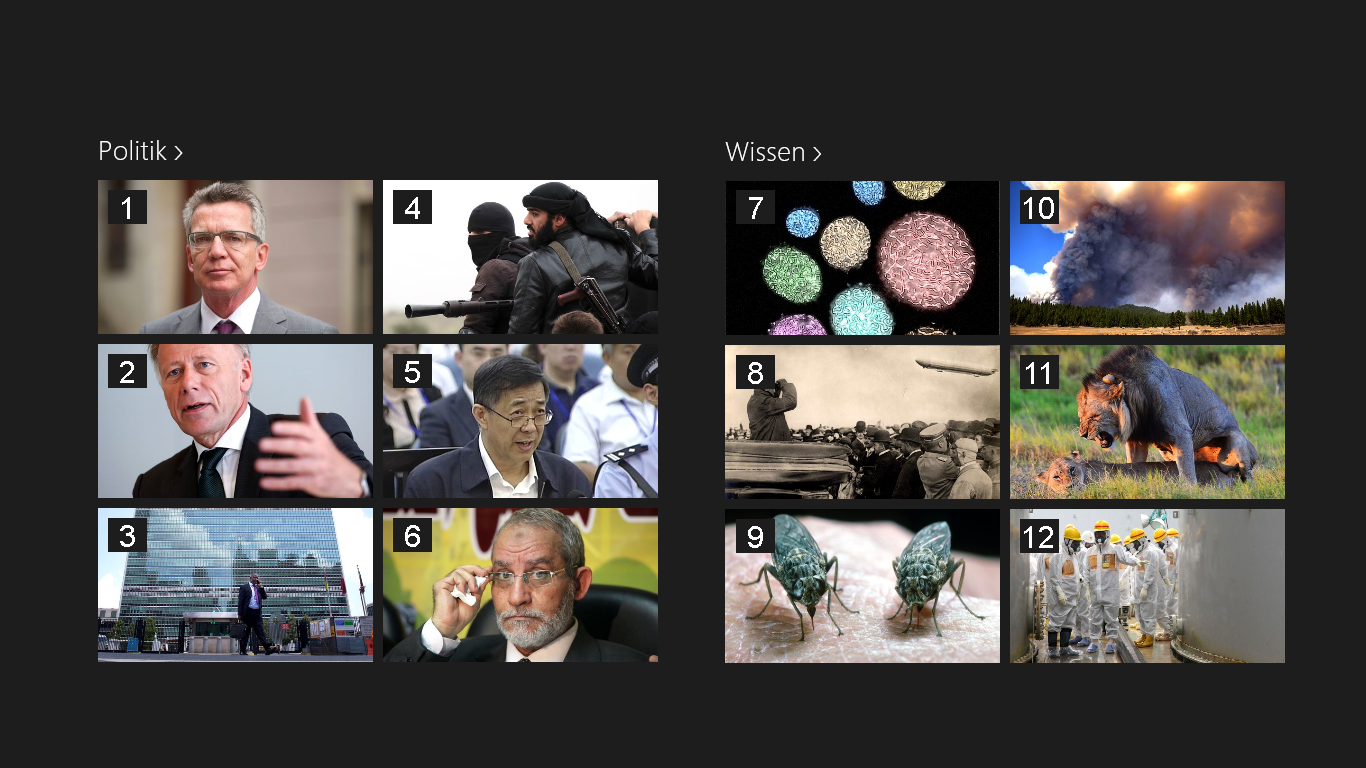
\includegraphics[width=\textwidth]{Evaluierung/Testbilder/collage_politik_wissen_numbers.png} 
	\caption{Die Testbilder aus dem Politik- und Wissen-Ressort.}
	\label{fig:testbilder}
\end{figure}  

Die Bilder sind nicht speziell zu diesem Zweck ausgewählt worden. Es handelt sich um die ersten sechs Artikel des jeweiligen Ressorts, wie sie am Sonntag, den 25. August 2013, auch auf der ZEIT ONLINE Webseite zu finden waren. Die Testpersonen sollen jedes Bild einzeln betrachten, zunächst eine Einschätzung zum groben Themengebiet geben und anschließend so genau wie möglich beschreiben, worum es in dem jeweiligen Artikel gehen könnte. Die Ergebnisse werden in einem Tabellenkalkulationsprogramm festgehalten.

Im zweiten Teil der Evaluierung sollen die Testpersonen die App benutzen: Zum einen auf einem Notebook, auf welchem die App mit der Maus bedient wird, und zum anderen auf dem \textit{Microsoft Surface}, ein Tablet, welches mit Touchgesten bedient wird. Es gibt vorher keine Instruktionen, wie die App zu bedienen ist. Die Testpersonen sollen die App selbst entdecken und mögliche Features, die programmiert wurden, finden und ausprobieren. Dies soll zeigen, wie intuitiv das Navigationskonzept und die Menüführung der App sind.

Die Evaluierung endet mit dem dritten Teil, einem Interview. Hier sollen im Gespräch einige Fragen zu den verschiedenen Teilen der Evaluierung beantwortet werden. Nachfolgend sind die Fragen aufgelistet, die im Einzelfall durch Nachfragen variiert werden können.

\begin{enumerate}
	\item Kannst du kurz deine bisherigen Erfahrungen mit Windows 8 schildern?
	\item In welcher Weise und wie oft konsumierst du Nachrichten im Allgemeinen? 
	\item Wie war dein Gedankengang, um herauszufinden, was sich hinter den Bildern verbergen könnte?
	\item Wie kamst du mit der App im Allgemeinen zurecht? War sie intuitiv? Welches Gerät hat dir besser gefallen und warum?
	\item Glaubst du der \glqq Nur-Bilder-Modus\grqq\ macht neugierig? Oder glaubst du er hemmt den Nachrichtenkonsum? 
\end{enumerate}

Um den Redefluss der Teilnehmer nicht zu unterbrechen, werden die Interviews als Audiomitschnitt gespeichert und später ausgewertet. Quelle der aufgeführten Zitate sind diese Mitschnitte, welche auf der beigelegten CD angehört werden können.

\subsection{Ergebnisse}
\label{subsec:ergebnisse}
Hier sollen die Ergebnisse der Evaluierung dargestellt und bewertet werden. Zunächst geht es um die App und ihr Benutzungs- bzw. Navigationskonzept. Anschließend wird der Ansatz untersucht, ob Nachrichten auch auf eine neue Art und Weise konsumiert und entdeckt werden können.

\subsubsection{Intuitivität der App} 
\label{subsubsec:intuitivitätderapp}
Ob die App für die einzelne Testperson intuitiv bedienbar ist, hängt mit bereits gesammelten Windows 8 Erfahrungen zusammen. TP3-TP5 gaben bei der Frage nach der bisherigen Windows 8 Erfahrung an, bisher nur im Desktop-Modus von Windows 8 gearbeitet zu haben. Dies geschah ausschließlich mit Maus und Tastatur. TP1 hat bereits erste Erfahrungen mit der Modern UI Oberfläche gemacht. Außerdem ist sie vertraut mit dem Smartphone-Betriebssystem von Microsoft, Windows Phone. TP2 hat bereits etwas tiefer gehende Erfahrungen mit Windows 8 und seinen Gesten, wenn auch hauptsächlich mit der Maus und weniger mit Touchbedienung.

TP1 fand das Navigationskonzept \glqq absolut intuitiv\grqq, wobei sie anmerkte, ihr hätte eine weitere Verbindung aus der Artikelansicht direkt zur Hubansicht gefallen. Klickt der User erst auf die Ressortübersicht und anschließend auf einen Artikel, kann nicht direkt zurück zur Hubansicht navigiert werden, sondern es muss der \glqq Umweg\grqq\ zurück über die Ressortübersicht genommen werden. TP2 meinte die App sei gut strukturiert, da diese Ebenenstruktur bekannt sei, merkte aber gleichzeitig an, dass er sich vorstellen kann, das \emph{Nicht} Windows 8 Nutzer zunächst Schwierigkeiten mit der Bedienung und den Gesten haben könnten. TP3 und TP4 fanden es etwas verwirrend, dass im Artikel horizontal gescrollt wird, im Gegensatz zu normalen Webseiten. TP5 \glqq fehlte die nötige Vertrautheit mit der Modern UI Oberfläche\grqq, um die nicht sofort sichtbaren Menüs aufzurufen. Die Texte hingegen seien sehr gut lesbar.

Generell lässt sich sagen, dass die Hauptnavigationsstruktur (Hubansicht, Ressortübersicht, Artikelansicht) von allen Testpersonen für intuitiv und gut verständlich empfunden wurde. Die meisten haben es auch geschafft, die Menüs mit den Features \glqq Titel ausblenden\grqq\ und \glqq Schriftgröße\grqq\ aufzurufen. Ein Feature wurde allerdings nur von einer Testperson gefunden, der \glqq Semantic Zoom\grqq. Wenn dieses Navigationselement von einer App benutzt wird, sollte gezielt darauf hingewiesen werden, da die Möglichkeit eines \glqq Semantic Zooms\grqq, gerade für Windows 8 Einsteiger, oft nicht intuitiv ersichtlich ist.

\subsubsection{Der Nur-Bilder-Modus}
\label{subsubsec:nurbildermodus}
Hier sollen die Möglichkeiten und die Sinnhaftigkeit des \glqq Nur-Bilder-Modus\grqq\  dargestellt und untersucht werden. Alle Testpersonen gaben an, täglich über verschiedenste Kanäle Nachrichten zu konsumieren, sei es im Fernsehen, Online, im Radio, über Smartphone oder durch die Zeitung. Damit ist zu vermuten, dass alle Testpersonen über ein Basiswissen, was tagesaktuelle Geschehnisse betrifft, verfügen.

Im ersten Teil der Evaluation sollten die Testpersonen versuchen herauszufinden, welcher Inhalt sich hinter den Teaserbildern von Abbildung \ref{fig:testbilder} verbergen könnte. Hierzu sollte zunächst ein grobes Themengebiet genannt werden und anschließend so genau wie möglich versucht werden zu bestimmen, worum es in dem jeweiligen Artikel konkret geht. Ein Bild wurde in diesem Fall als \glqq genau\grqq\ akzeptiert, wenn die Testpersonen nach der allgemeinen Einordnung auch noch die konkreten Themen der jeweiligen Artikel benennen konnten. So wurde es z.B. als richtig akzeptiert, wenn die Testperson bei Bild 10 nicht nur das grobe Thema \glqq Waldbrände\grqq, sondern auch \glqq San Francisco\grqq\ oder \glqq Yosemite Nationalpark\grqq\ richtig benannt hatte. Nach diesem Bewertungsschema wurden von den 12 Bildern im Durchschnitt 78\% grob und 35\% auch genauer richtig zugeordnet. Das am häufigsten richtig zugeordnete Bild ist Bild 10. Es wurde von allen Testpersonen genau richtig erkannt, dicht gefolgt von Bild 5, welches von 4 Testpersonen genauer richtig zugeordnet werden konnte und von einer Testperson nur grob. Am wenigsten konnten die Testpersonen mit Bild 3 anfangen, es wurde nur von einer Testperson erkannt, dafür aber auch genau. Es geht in diesem Bild um die NSA-Affäre und den UN-Sicherheitsrat. Eine Übersicht mit allen zugehörigen Artikel-Schlagzeilen befindet sich im Anhang \ref{app:anhangA}.

Die Testpersonen wurden im Interview gefragt, wie sie an diese Aufgabe herangegangen sind. In einem Punkt waren sich alle Testpersonen einig. Wenn nur eine Person abgebildet ist, müssen weitere Informationen über andere Nachrichtenkanäle bekannt sein, um den Inhalt genauer zu erkennen. TP1 meint, bei Bild 1 sei es sehr schwer, etwas genaues sagen zu können, da diese Person für verschiedene Themen in Frage kommt, z.B. Euro Hawk, Afghanistan, Syrien oder Strukturänderung Bundeswehr. TP5 sagt zu Bild 6: \glqq Bei Bildern, auf denen keine öffentlichen Personen drauf waren, hab ich einfach versucht, über Vorurteile die Personen zu lesen\grqq. 

Bei den Bildern aus dem Politik-Ressort wurde oft auf das bereits aus anderen Nachrichtenquellen Gehörte zurückgegriffen, wohingegen bei den eher zeitlosen Artikeln und Bildern wie z.B. Bild 8 und Bild 11 die grobe Zuordnung recht leicht fiel, aber das Bild für die genaue Bestimmung nicht genügend Informationen lieferte und die Testpersonen auch nicht mit tagesaktuellem Wissen auf die konkreten Inhalte schließen konnten. Bei Bild 8 geht es z.B. darum, dass Graf Zeppelin angeblich gar nicht der Erfinder des Zeppelins war, und bei Bild 11 lautet der Titel: \glqq Hat nur der Mensch Sex in der Missionarsstellung?\grqq. 

Es bleibt noch zu klären, ob ein \glqq Nur-Bilder-Modus\grqq\ sinnvoll ist und inwieweit der User dadurch neugierig gemacht wird oder ob dieser Modus ihn eher in seinem Nachrichtenkonsumfluss stört und hemmt. TP1 sagt dazu: \glqq Das kommt drauf an, was ich gerade möchte, [...] wenn ich mich kurz und prägnant informieren möchte [...] muss unbedingt der Text drin sein, [aber] wenn ich mal ein bisschen Zeit habe und sitze irgendwo und warte, dann ist es eher der Entdeckermodus\grqq. TP2 meint, es hänge von der Veranlagung der Person ab. Es sei eine offene Herangehensweise nötig: \glqq Ich gucke mal was mir angeboten wird\grqq. Weiterhin glaubt TP2, dass Inhalte so eventuell besser im Gedächtnis bleiben, weil der User auf diese Weise aktiv auf ein Bild, welches seine Neugier geweckt hat, klickt und sich damit den Inhalt gewissermaßen selbst \glqq erarbeitet\grqq\ hat. TP4 sieht es ähnlich wie TP1. Es komme auf die Situation an und das Ziel des Nachrichtenkonsums an. TP5 meint, es hänge auch sehr stark vom jeweiligen Bild ab: \glqq Es muss eine klare Verbindung zum Inhalt geben [,um die Neugier zu wecken,] was bei reinen Personenbildern nicht der Fall ist.\grqq. 

Die Testpersonen stimmen bei dieser Frage grundlegend überein. Wenn der User gezielt tagesaktuelle Nachrichten konsumieren will, ist ein \glqq{Nur-Bilder-Modus\grqq\ nicht zielführend. Es muss zu viel geraten und vermutet werden, im Zweifel klickt der User auf ein Bild, hat aber etwas ganz anderes erwartet und auf diese Weise ein Negativ-Erlebnis. Hat der User andererseits ein bisschen mehr Zeit und möchte mal etwas Neues ausprobieren, sich durch die Nachrichtenwelt treiben lassen, dann stellt der \glqq{Nur-Bilder-Modus\grqq\ eine interessante Alternative dar. Hier kann sich der User ganz auf seinen Neugier- und Entdeckertrieb verlassen und prüfen, ob er mit seiner aus dem Bild abgeleiteten Vermutung über den Artikelinhalt tatsächlich richtig liegt. Der Trend zeigt deutlich: Um den \glqq{Nur-Bilder-Modus\grqq\ genießen zu können, sollte der User etwas Zeit mitbringen und sich bewusst darauf einlassen, nicht auf den ersten Blick alle Informationen dargelegt zu bekommen.

Zusammenfassend lassen sind folgende Punkte zum \glqq Nur-Bilder-Modus\grqq\ feststellen. Um aus den Bildern auf Inhalte schließen zu können, müssen Basiskenntnisse aus anderen Nachrichtenquellen vorhanden sein. Auf die groben Inhalte der Artikel kann bei den meisten Bildern geschlossen werden, sowohl bei den aktuellen als auch bei zeitlosen Artikeln. Bei Bildern, auf denen nur Personen dargestellt sind, ist es schwierig, inhaltliche Details bestimmen. Des Weiteren gelingt Identifizierung von genauen Inhalten eher für aktuelle Themen. Für den gezielten Nachrichtenkonsum wird die Kombination von Bild und Text bevorzugt. Der \glqq Nur-Bilder-Modus\grqq\ funktioniert nur, wenn der Leser genügend Zeit und Interesse mitbringt.

\newpage
\section{Fazit}
\label{sec:fazit}
Nachdem die ZEIGHT App konzeptioniert, umgesetzt und evaluiert wurde, soll festgestellt werden, inwieweit die formulierten Ziele der App und der gesamten Arbeit umgesetzt wurden.

Es sollte eine intuitive und ansprechende Nachrichten App entwickelt werden. Durch das hierarchische Navigationssystem und das Einsetzen von Menüleisten gliedert sich die App in das \glqq Look \& Feel\grqq\ von Windows 8 ein. Die Evaluierung hat gezeigt, dass die App intuitiv bedienbar ist. Lediglich bei den Windows 8 spezifischen Gesten, gab es vereinzelt Schwierigkeiten aufgrund mangelnder Erfahrung mit dem System.

Des Weiteren sollte eine Umgebung geschaffen werden, die es erlaubt die  Nachrichten auf der Einstiegsebene rein visuell zu erleben, um anschließend untersuchen zu können, ob so ein Modus sinnvoll ist. Diese Funktionalität wurde umgesetzt, indem eine Funktion zum Aus- und Einblenden der Artikeltitel implementiert wurde. In der Evaluierung wurde untersucht, inwieweit nur aus Bildern auf die jeweiligen Themen der Artikel geschlossen werden kann mit dem Ergebnis, dass die meisten Bilder grob zugeordnet werden können. Hierbei hat sich gezeigt, dass ein \glqq Nur-Bilder-Modus\grqq\ nur in bestimmten Situationen Sinn macht. Möchte sich der User gezielt über die aktuelle Nachrichtenlage informieren, werden ihm hierfür im \glqq Nur-Bilder-Modus\grqq zu wenig Informationen geliefert. Bringt der User mehr Zeit zum Konsumieren der Nachrichten mit, hat sich gezeigt, dass der rein visuelle Modus eine interessante Alternative darstellt. Der User kann auf diese Weise die Nachrichten eher entdecken als sie \glqq nur\grqq\ zu konsumieren. Die ZEIGHT App ist für beide Herangehensweisen flexibel einsetzbar.

Zusammenfassend kann gesagt werden, dass die Ziele dieser Arbeit und der App erfüllt wurden. 

Abschließend wird ein Ausblick auf die Zukunft von ZEIGHT gegeben. Im allgemeinen wird erwartet das Windows 8 innerhalb der Windows Welt immer mehr an Bedeutung gewinnt\footnote{Quelle: http://winfuture.de/news,77692.html}. Bei zunehmender Akzeptanz dieses Betriebssystems am Markt wäre dann zu untersuchen, ob für eine ZEIT ONLINE Nachrichten App unter Windows 8 ein geeignetes Finanzierungsmodell entwickelt werden kann.

\newpage
\begin{singlespace}
	\bibliographystyle{natdin}
	\bibliography{ba_literatur}
\end{singlespace}

\newpage
\appendix
\pagenumbering{roman}
\thispagestyle{plain}

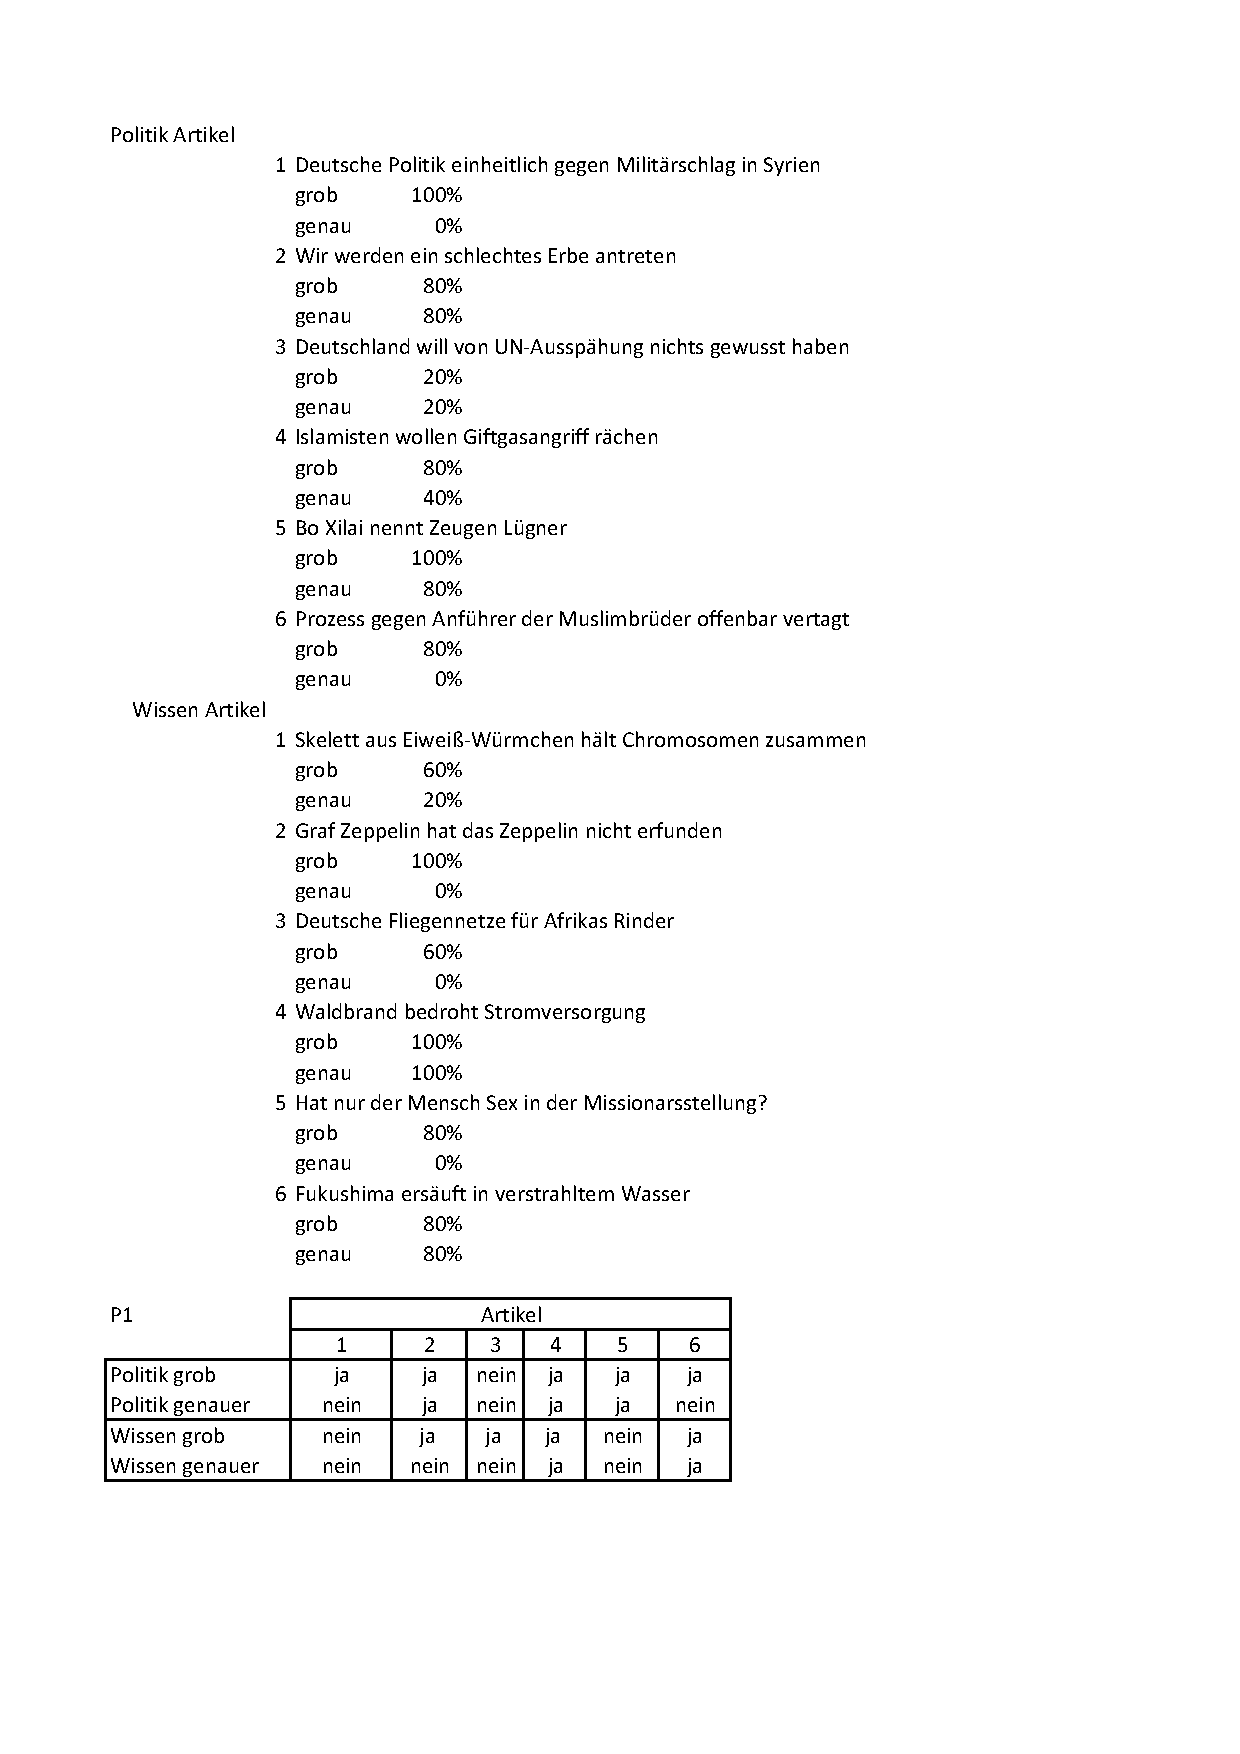
\includepdf[pages=1,scale=.9,pagecommand={\section{Detaillierte Evaluierung Bild-Inhalt Relation} \label{app:anhangA}}]{Evaluierung/rel_bilder_inhalt.pdf}

\includepdf[pages=2,scale=.9,pagecommand={}]{Evaluierung/rel_bilder_inhalt.pdf}

\section{CD Inhalt}
\label{app:cd}
Folgende Dateien sind auf der beigelegten CD enthalten:

\begin{itemize}
	\item Die Bachelorthesis als PDF-Datei
	\item Die Bachelorthesis als LaTeX Projekt
	\item Die ZEIGHT App als Visual Studio Projekt
	\item Die digitale Version von Anhang \ref{app:anhangA}, inklusive Excel Datei
	\item Die Audiomitschnitte der Interviews
	\item Ein Video, welches die ZEIGHT App zeigt und ihre Funktionen erklärt
\end{itemize}

\newpage
\section*{Eigenständigkeitserklärung}
\thispagestyle{empty}
Ich versichere, die vorliegende Arbeit selbständig ohne fremde Hilfe verfasst und keine anderen Quellen und Hilfsmittel als die angegebenen benutzt zu haben. Die aus anderen Werken wörtlich entnommenen Stellen oder dem Sinn nach entlehnten Passagen sind durch Quellenangaben eindeutig kenntlich gemacht.
\vspace{3cm}
\begin{tabbing}
\hspace{6cm}  \= \kill
\textit{Hamburg, 03.09.2013} \> \textit{Malte Modrow}
\end{tabbing}
\end{document}